\documentclass[12pt,a4paper]{book}

\usepackage{fontspec}
\setmainfont{Geneva} % Geneva, Helvetica, Helvetica Neue
\usepackage{xunicode}
\usepackage{polyglossia}
\setmainlanguage{french}
\setotherlanguage{english}
\usepackage[maxlevel=3]{csquotes}
\usepackage{frcursive}
\usepackage{pifont}
\renewcommand{\footnoterule}{%
\vspace*{0.2cm}%
\ding{47}\hfill \centering Notes\hfill \ding{45}\vspace*{.2cm}\hrule\vspace*{.2cm}}

\usepackage{xcolor}
\newcommand{\exEN}[1]{%
  \textcolor{blue}{\textenglish{#1}}}
\newcommand{\exFR}[1]{%
  \textcolor{olive}{\textcursive{#1}}}

\renewcommand{\mkcitation}[1]{\footnote{#1}}
\renewcommand{\mktextquote}[6]{#1#2#6#4#3#5}

\usepackage{hyperref}
\begin{document}
\title{La phonétique anglaise comparée à la française}
\hypersetup{
 pdfauthor={Laurent Garnier},
 pdftitle={45 Phonetic Sounds of English},
 pdfkeywords={},
 pdfsubject={},
 pdfcreator={Emacs 25.3.1 (Org mode 9.1.6)}, 
 pdflang={English}}
\author{Laurent Garnier}

\maketitle
\tableofcontents

\part{Introduction}

\chapter{Introduction}
\label{sec:org9288afb}
Dans cet ebook (ou livre électronique en bon français), vous allez
découvrir ce qui est bien trop souvent passé sous silence dans les
cours de langues\ldots{}, la phonétique ! En effet, en France en
particulier\footnote{N'ayant jamais fait d'études à l'étranger je ne
  peux pas me permettre de parler des autres pays}, les cours de
langues insistent rarement sur l'oral. Attention, je parle des cours
de langue avant le bac. Il faut savoir que \emph{normalement}
l'objectif de l'enseignement obligatoire\footnote{En France
  l'instruction est obligatoire jusqu'à 16 ans ce qui correspond
  normalement à la classe de seconde ou première en cas de
  redoublement.} est d'atteindre le
\href{http://www.cambridgeenglish.org/fr/exams-and-tests/cambridge-english-certificate-cec/}{niveau
  B1} du cadre de référence européen. Hélas, la réalité est
loin d'être celle qu'espèrent les ministres et de nombreux indicateurs le prouvent :
\begin{itemize}
\item niveau en anglais par rapport aux autres pays
  \href{https://www.ef.fr/epi/regions/europe/}{européens}\footnote{Vous
    pouvez aller directement sur le site
    \url{https://www.ef.fr/epi/regions/europe/} pour observer l'étude complète.}(derrière l'Espagne, la Grèce, la Bulgarie, la Roumanie\ldots{} voir la figure
  \ref{fig:1} page \pageref{fig:1} pour plus de détails)
  \begin{figure}[h]
    \centering
    \caption[L'anglais en Europe]{Niveau d'anglais des
      pays européens}\vspace{.1cm}
    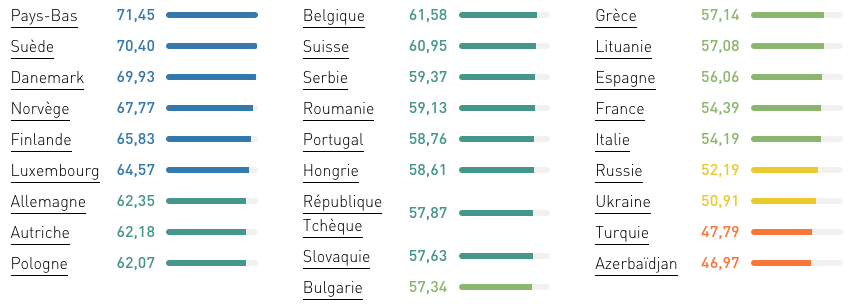
\includegraphics[scale=.5]{french-english-level-in-europe}
    
    \label{fig:1}
  \end{figure}
\item niveau en anglais par rapport \href{https://www.ef.fr/epi/}{au
    reste du monde}\footnote{Vous pouvez aller directement sur le site
  \url{https://www.ef.fr/epi/} pour observer l'étude complète}
(derrière la République Dominicaine et la Corée du Sud s'il vous
plaît\ldots{} voir la figure \ref{fig:2} page \pageref{fig:2} pour
plus de détails)
  \begin{figure}[h]
    \centering
    \caption[L'anglais dans le monde]{Niveau d'anglais dans le monde}\vspace{.1cm}
    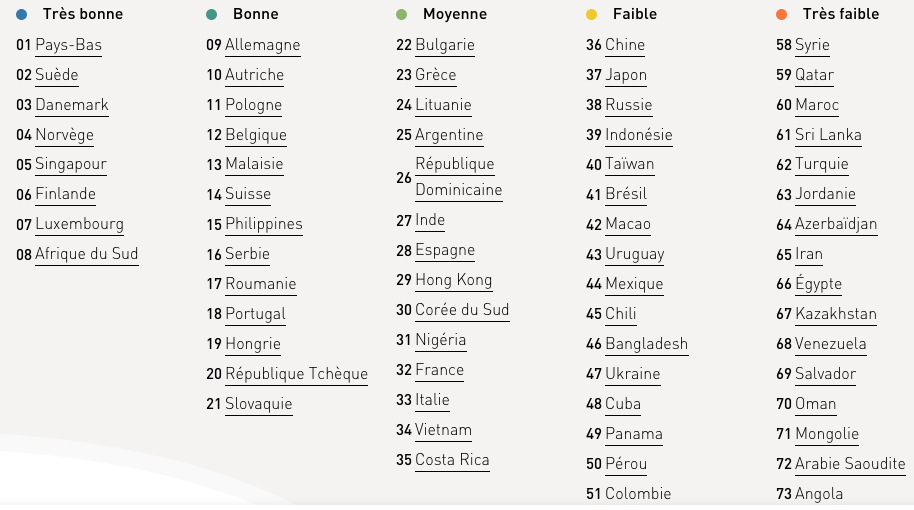
\includegraphics[scale=.5]{english-level-in-the-world}
    
    \label{fig:2}
  \end{figure}
\item encore des
  \href{https://www.digischool.fr/international/tests-anglais/chiffres-cles-francais-langues-etrangeres-16265.html}{chiffres
    accablants}\footnote{Vous pouvez lire l'article complet sur le
    site
    \url{https://www.digischool.fr/international/tests-anglais/chiffres-cles-francais-langues-etrangeres-16265.html}}
    (1/5 des français parlent anglais couramment voir la figure
    \ref{fig:3} page \pageref{fig:3} pour plus de détails.)
  \begin{figure}[h]
    \centering
    \caption[L'anglais en France]{Niveau d'anglais en France}\vspace{.1cm}
    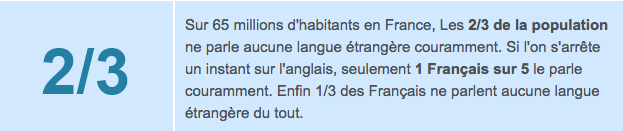
\includegraphics[scale=.725]{french-english-level-in-france}
    
    \label{fig:3}
  \end{figure}
\end{itemize}
Loin de moi l'idée de vous assommer avec des chiffres et encore moins
de partir dans l'auto-flagellation. Néanmoins, il faut être lucide, il
y a un problème franco-français (qui est très bien expliqué dans cet
\href{http://www.larevuedesressources.org/les-francais-et-les-langues-etrangeres,2920.html}{essai}). 
Ce problème est très bien développé et analysé dans l'essai du
professeur Daniel Emilio Rojas\footnote{Lisez-le c'est gratuit, très
  bien écrit et instructif : \url{http://www.larevuedesressources.org/les-francais-et-les-langues-etrangeres,2920.html}} (hispanophone natif qui parle et écrit
probablement beaucoup mieux le français que 90\% d'entre
nous). Cependant, je me permettrais de vous proposer un raccourci
(forcément réducteur) pédagogique en vous rappelant un fait
élémentaire mais que l'on oubli trop souvent. Parfois les solutions
sont tellement \emph{bêtes} qu'on oubli d'y penser. Attention, je ne
prétends pas vous proposer de recette miracle. L'anglais est une
langue difficile\footnote{C'est Claude Hagège, linguiste et professeur
  au Collège de France, qui l'explique dans cette vidéo
  \url{https://youtu.be/fjAuHvOMXFE} }, bizarre, complexe et illogique
(comme beaucoup de langues et notamment le français); et je ne suis
pas le seul à le dire puisque certains anglophones natifs (et
linguistes de surcroît) le disent et l'écrivent dans cet \href{https://aeon.co/essays/why-is-english-so-weirdly-different-from-other-languages}{article} qui permet également d'être
écouté\footnote{Comme je le montre dans cette vidéo
  \url{https://youtu.be/6wLbtx2iL7c}}. Donc oui l'anglais est
difficile, \textbf{mais} avec un peu de bon sens et de persévérence
vous pouvez y arriver\footnote{Bon, il y a une triste vérité qu'il
  faut accepter, vous ne parlerez \textbf{jamais} comme un natif (sauf
  si vous décidez de vous installer dans un pays anglophone), mais
  vous serez à l'aise et tout le monde vous comprendra quand même si
  vous pratiquez régulièrement}. 

Mais quel est donc ce truc \emph{tout bête} que l'on oublierait et dont je
ne vous ai toujours pas parlé ? Minute papillon ! Non ! Je n'essaie
pas de noyer le poisson, je vais vous révéler mon \emph{truc}. Je vous
préviens, vous allez être probablement déçu, mais pourtant c'est une
évidence. \par
Allons-y ! Et bien, je ne sais pas pour vous mais pour moi (et il me
semble pour la plupart des gens aussi), l'acquisition de ma langue
maternelle a commencé par l'oral et non par l'écrit. Pendant au moins
5 ans (avant de rentrer au CP ou tout autre système scolaire qui
apprend à lire et à écrire), j'ai pratiqué en priorité l'écoute et la
méthode essai/erreur (en anglais on dit \emph{try and guess} ce qui veut
dire \emph{essayer et deviner}, qui est un point de vue plus positif). Ben
oui, quand on est enfant on baigne dans un environnement linguistique
oral. Et dès les premiers mois de la vie on essaie (avec beaucoup de
difficultés au début) de produire ou plutôt reproduire des sons que
l'on a entendu. Et croyez-moi, si vous avez oublié allez faire un tour
chez votre frère, soeur, cousin, cousine, ami, amie qui a (ont) des
enfants en bas âge et cela vous raffraichira la mémoire. La parole est
si importante pour l'humanité qu'elle a été pendant des siècles ( des
millénaires même!) le seul et unique vecteur de
communication. D'ailleurs aujourd'hui encore parmi les presque 7~000
\href{http://www.museedelhomme.fr/fr/combien-langues-sont-parlees-monde}{langues dans le monde} la plupart ne possèdent pas de système
d'écriture. Pour plus de précisions sur la répartition linguistique
dans le monde vous pouvez consulter \href{http://www.axl.cefan.ulaval.ca/Langues/1div\_recens.htm}{ce site canadien} qui tire ses
sources statistiques du \textbf{Summer Institute of Linguistics} du
Texas\footnote{Voici l'url du site
  \url{http://www.axl.cefan.ulaval.ca/Langues/1div_recens.htm}}
(2017).\par


\begin{quote}
Les Romains, déjà, ne parlaient pas exactement la langue qu'ils
écrivaient. Ainsi, \emph{cheval} vient d'un mot parlé, \emph{caballus}, alors
que le latin classique écrit \emph{equus} -- d'où viendront des mots <<~savants~>> comme \emph{équidé} et \emph{équitation}
\end{quote}\footnote{Extrait du livre \href{https://www.amazon.fr/gp/product/2844100015/ref=as\_li\_tl?ie=UTF8\&camp=1642\&creative=6746\&creativeASIN=2844100015\&linkCode=as2\&tag=wwwbecomefree-21\&linkId=985f3a849fd44728e8480993cf2d5490}{français lycée} de Pierre Brunel.}

D'ailleurs comme le montre \href{https://youtu.be/Wn\_eBrIDUuc}{cette vidéo}, les zones du cerveau actives
pour la parole et pour l'écriture sont différentes.\par

\begin{quote}
Longtemps, le français s'est écrit comme il se parlait; vice versa,
toutes les lettres se prononçaient, comme en latin. La notion même
d'orthographe n'existait pas.
\end{quote}\footnote{Extrait du livre
\href{https://www.amazon.fr/gp/product/2844100015/ref=as\_li\_tl?ie=UTF8\&camp=1642\&creative=6746\&creativeASIN=2844100015\&linkCode=as2\&tag=wwwbecomefree-21\&linkId=985f3a849fd44728e8480993cf2d5490}{français
  lycée} de Pierre Brunel.}


En lisant cet extrait je pari que certains d'entre vous sont en train
de chercher un moyen pour inventer une machine à remonter le temps. 

Vous vous demandez sûrement où je veux en venir. Mon but est de vous
faire comprendre ou plutôt de vous rappeler qu'une langue ça s'écoute
et ça se parle pendant un certain temps (jusqu'à ce que ça devienne
naturel) avant d'apprendre à l'écrire et d'étudier toutes les
subtilités de la grammaire. \href{https://fr.wikipedia.org/wiki/Django\_Reinhardt}{Django Reinhardt} et \href{https://fr.wikipedia.org/wiki/Louis\_Armstrong}{Louis Amstrong} ne
savaient ni lire ni écrire la musique et pourtant ils sont des
musiciens vénérés de leur vivant et encore aujourd'hui.\par

Et oui une langue c'est également une musique ! Une langue a une
musicalité et un rythme. Pas de chance pour nous le français (ou
plutôt le \emph{parisien}\footnote{Les langues d'oc plus proches du
  latin étaient bien plus riches, et même parmi les langues d'oïl le
  parisien n'était pas spécialement la plus efficace par rapport au
  picard notamment.})
n'est pas très chantant. Mais pourtant si l'on écoute les accents du
midi il y a tout de suite plus de mélodies qui chatouillent nos
oreilles. 

En résumé, ce que je vais partager avec vous dans ce livre, ce
sont les sons de la langue anglaise. Les 45 sons (certains en
décrivent 44, pour le français\footnote{Selon le
  \href{https://www.amazon.fr/gp/product/221010632X/ref=as_li_tl?ie=UTF8&camp=1642&creative=6746&creativeASIN=221010632X&linkCode=as2&tag=wwwbecomefree-21&linkId=c8c522ee07ffc9188dd9a768e39d88e0}{Grévisse
  de l'enseignant} il y a 36 sons <<~\emph{purement}~>> français
auquel on ajoute le son [ŋ] hérité de l'anglais et notamment utilisé dans \emph{parking}.} c'est pareil, certains disent 36
d'autres 37). Je vais vous présenter ces 45 sons qui sont absolument
\textbf{fondamentaux}. En insistant particulièrement sur ceux qui
n'apparaissent pas du tout dans la langue française. Et pour bien
faire la différence on commencera par la phonétique de la langue
française que vous ne connaissez probablement pas encore.\par

J'ai dit qu'on apprend d'abord à parler avant d'écrire, c'est vrai,
mais a priori, si vous lisez ce livre c'est que vous savez lire. Et
comme vous savez lire et bien on va en profiter pour apprendre encore
plus efficacement en utilisant
l'\href{https://fr.wikipedia.org/wiki/Alphabet\_phon\%25C3\%25A9tique\_international}{API}\footnote{Vous
pouvez le consulter sur Wikipédia \url{https://fr.wikipedia.org/wiki/Alphabet_phon\%C3\%A9tique_international}}
(Alphabet Phonétique International). En anglais on l'écrit
IPA\footnote{Vous pouvez également consulter la version anglaise de
  Wikipédia \url{https://en.wikipedia.org/wiki/International_Phonetic_Alphabet}}
(International Phonetic Alphabet).\par

Et cerise sur le gâteau, ceci
vous sera utile pour toutes les autres langues que vous souhaitez
apprendre ou que vous parlez déjà (cela va même améliorer votre
français\footnote{Vous pouvez déjà vous entraîner grauitement grâce
  aux cartes mémoires que j'ai créé : \url{https://tiny.cards/decks/6YTEvyrN/english-phonetics}} !). D'ailleurs, contrairement à ce que certaines personnes
pourraient penser, apprendre une autre langue, et en particulier
l'anglais, améliore votre niveau de français\footnote{En effet il existe plus de 25~000 mots anglais
  d'origine française et vous pouvez en découvrir quelques-uns grâce
  aux cartes mémoires que j'ai créé :
  \url{https://tinycards.duolingo.com/decks/6VNKUdba/english-words-with-french-origin}
et au livre plus complet \href{https://www.amazon.fr/gp/product/225315444X/ref=as_li_tl?ie=UTF8&camp=1642&creative=6746&creativeASIN=225315444X&linkCode=as2&tag=wwwbecomefree-21&linkId=5317e7b0e063b4d6c7c676b11420e49d}{Honni soit qui mal y pense} }. Ce n'est pas magique,
mais c'est véridique. Alors c'est parti, allons découvrir les 45 sons
de la langue anglaise (qui n'a plus grand chose à voir avec
Shakespeare de la même manière qu'on ne parle plus la langue de
Molière).

\part{Phonétique du français}
\chapter{Voyelles}\label{chap:voy}
Que celui ou celle qui a dit <<~consonne~>> juste après avoir lu le
titre du chapitre sorte immédiatement\footnote{Toute référence à une
  émission de la télévision française serait purement fortuite, un
  coup du hasard si j'ose pousser légèrement la prose.}!\par
Plus sérieusement, lorsqu'on regroupe les voyelles\footnote{Puisque ce
  livre parle de phonétique on s'occupe des sons donc de l'oral et pas
  de l'écrit (donc on se fiche qu'il y ait six voyelles écrites).} on
découvre deux grandes catégories : les voyelles dites \emph{Orales} et
les voyelles dites \emph{Nasales}\footnote{Que les anglophones ont du
  mal à prononcer correcement.}.

Un son de voyelle est fait en façonnant l'air comme il quitte la
bouche. Nous utilisons les articulateurs pour façonner l'air - les
lèvres, la mâchoire, la langue. La langue française parlée compte
ainsi seize voyelles, 12 orales et 4 nasales.

\section{Voyelles orales}\label{sec:orales}
\subsection{Le son [a]}\label{subsec:afr}

C'est le son que l'on trouve dans les mots \exFR{arrêt} (/aʀɛ/),
\exFR{bar} (/baʀ/), \exFR{chat} (/ʃa/), et bien
d'autres. 

Observons un exemple pour chacun d'entre eux et voyons leurs
traductions anglaises :\par

\begin{enumerate}
\item \exFR{arrêt} (/aʀɛ/)
  \begin{itemize}
  \item \exFR{Ce matin j'ai attendu à l'arrêt de
      bus pendant dix  minutes.}
    \item \exEN{This morning I waited at the bus stop for ten minutes.}
    \end{itemize}
    Le mot \exEN{stop} est même utilisé dans la langue française
    au point que certaines personnes le conjuguent (\textquote[][.]{\exFR{J'ai stoppé net quand j'ai vu la voiture arriver}}).
    Cependant en anglais on
    prononce
    \href{https://en.oxforddictionaries.com/definition/stop}{/stɒp/}
    alors qu'en français on le prononce
    \href{http://www.wordreference.com/fren/stop}{/stɔp/}\footnote{Les
      sons [ɒ] et [ɔ] sont bien distincts}.
\item \exFR{bar} (/baʀ/)
  \begin{itemize}
  \item \exFR{Dans la rue où j'ai grandi il y
      avait un bar juste en bas de chez moi.}
  \item \exEN{In the street where I grew up there was a bar just down from my house.}
  \end{itemize}
    Attention ! Les deux mots sont homographes\footnote{Deux mots sont
      dits homographes s'ils s'écrivent de la même manière (avec les
      mêmes lettres).} mais ils ne sont pas homophones\footnote{Deux
      mots sont dits homophones s'ils se prononcent de la même façon
      (même son).} ! En effet, en anglais on prononce
    \href{https://en.oxforddictionaries.com/definition/bar}{/bɑː/}
    alors qu'en français on dit \href{http://www.wordreference.com/fren/bar}{/baʀ/}; voilà un exemple qui illustre parfaitement l'intérêt
    d'étudier la phonétique.
  \item \exFR{chat} (/ʃa/)
    \begin{itemize}
    \item \exFR{Le chat des voisins vient souvent nous rendre visite.}
    \item \exEN{The neighbor's cat often comes to visit us.}
    \end{itemize}
    Ici on a d'une part \exFR{chat} qui se prononce
    \href{http://www.wordreference.com/fren/chat}{/ʃa/} en français et
    \exEN{cat} en anglais qui se prononce
    \href{http://www.wordreference.com/enfr/cat}{/kæt/}. Attention !
    Le verbe anglais \exEN{to chat}\footnote{\exEN{To chat} signifie
      bavarder.} se prononce
    \href{https://en.oxforddictionaries.com/definition/chat}{/tʃæt/}. 
\end{enumerate}

\subsection{Le son [ɑ]}\label{subsec:ɑfr}

C'est le son que l'on trouve dans les mots \exFR{bâton} (/bɑtɔ̃ /),
\exFR{mât} (/mɑ/), \exFR{pâte} (/pɑt/), et bien d'autres.

Observons un exemple pour chacun d'entre eux et voyons leurs
traductions anglaises :\par

\begin{enumerate}
\item \exFR{bâton} (/bɑtɔ̃ /)
  \begin{itemize}
  \item \exFR{Souvent dans la liste des fournitures scolaires on demande
      un bâton de colle.}
    \item \exEN{Often in the list of school supplies we ask for a stick of glue.}
    \end{itemize}
    Le mot \exEN{stick}\footnote{Le mot \exEN{stick} signifie \exFR{bâton} et
      peut aussi vouloir dire \exFR{matraque}.} se prononce en anglais \href{https://en.oxforddictionaries.com/definition/stick}{/stɪk/}.
\item \exFR{mât} (/mɑ/)
  \begin{itemize}
  \item \exFR{Avant l'invention du moteur les bateaux étaient tous à
      voile et par conséquent il fallait bien que quelqu'un grimpe au
      sommet du mât pour l'accrocher.}
  \item \exEN{Before the invention of the engine the boats were all sailing and therefore it was necessary that someone climbs to the top of the mast to hang it.}
  \end{itemize}
  En anglais le mot \exEN{mast} se prononce
  \href{https://en.oxforddictionaries.com/definition/mast}{/mɑːst/}. En
  quelques sortes on peut dire qu'il est une prolongation sonore de son
  équivalent français.

  \item \exFR{pâte} (/pɑt/)
    \begin{itemize}
    \item \exFR{Pour faire des crêpes il faut d'abord préparer la pâte.}
    \item \exEN{To make pancakes it is necessary to first prepare the dough.}
    \end{itemize}
    On notera que le mot français \exFR{pâte}\footnote{Vous pouvez consulter
      directement les traductions disponibles sur \url{http://www.wordreference.com/fren/p\%C3\%A2te}} admet de nombreux
    équivalents anglais \exEN{pastry} (pour les tartes ou
    pâtisseries), \exEN{dough} (pour le pain et les crêpes),
    \exEN{base} (pour les pizzas) et j'en passe et des meilleurs ! 
\end{enumerate}

\subsection{Le son [e]}\label{subsec:efr}

C'est un son que l'on trouve par exemple dans les mots \exFR{créer}
(/kʀee/), \exFR{pré} (/pʀe/), \exFR{république} (/ʀepyblik/), et bien d'autres.

Observons un exemple pour chacun d'entre eux et voyons leurs
traductions anglaises :\par

\begin{enumerate}
\item \exFR{créer} (/kʀee/)
  \begin{itemize}
  \item \exFR{Créer est un acte souvent solitaire mais qui s'appuie
      également sur les travaux des autres.}
    \item \exEN{Creating is often a lonely act, but it is also based on the work of others.}
    \end{itemize}
    Le verbe anglais \exEN{create} se prononce
    \href{https://en.oxforddictionaries.com/definition/create}{/kriːˈeɪt/}.
\item \exFR{pré} (/pʀe/)
  \begin{itemize}
  \item \exFR{Dans le pré il y a les vaches qui broutent de l'herbe.}
  \item \exEN{In the meadow there are cows grazing grass.}
  \end{itemize}
  

\item \exFR{république} (/ʀepyblik/)
  \begin{itemize}
  \item \exFR{La France est une république.}
  \item \exEN{France is a republic.}
  \end{itemize}
  Même si les deux mots se ressemblent beaucoup graphiquement, ils
  ne se prononcent pas de la même manière. En effet, le mot
  \exEN{republic} se prononce \href{https://en.oxforddictionaries.com/definition/republic}{/rɪˈpʌblɪk/}. 
\end{enumerate}

  
\subsection{Le son [ɛ]}\label{subsec:ɛfr}

C'est un son que l'on trouve par exemple dans les mots \exFR{carrière}
(/kaʀjɛʀ/), \exFR{mère} (/mɛʀ/), \exFR{taire} (/tɛʀ/), et bien d'autres.

Observons un exemple pour chacun d'entre eux et voyons leurs
traductions anglaises :\par

\begin{enumerate}
\item \exFR{carrière} (/kaʀjɛʀ/)
  \begin{itemize}
  \item \exFR{Généralement les sportifs de haut niveau finissent leur
      carrière avant 40 ans.}
    \item \exEN{Generally top athletes finish their career before 40 years.}
    \end{itemize}
    Le mot français \exFR{carrière} est polysémique\footnote{Il a
      plusieurs significations différentes.} mais en anglais chaque
    sens du mot français\footnote{Vous pouvez en consulter une liste
      ici \url{http://www.wordreference.com/fren/carri\%C3\%A8re}.}  correspond à un mot différent. Par exemple
    \exEN{quarry}
    (\href{https://en.oxforddictionaries.com/definition/quarry}{
      /ˈkwɒrɪ/}) pour les carrières de pierres ou encore \exEN{career}
    (\href{https://en.oxforddictionaries.com/definition/career}{/kəˈrɪə/})
    pour la carrière professionnelle.
\item \exFR{mère} (/mɛʀ/)
  \begin{itemize}
  \item \exFR{C'est à toutes les mères que je dédicace ce livre.}
  \item \exEN{It is to all the mothers that I dedicate this book.}
  \end{itemize}

  
\item \exFR{taire} (/tɛʀ/)
  \begin{itemize}
  \item \exFR{Parfois pour plaire il vaut mieux se taire.}
  \item \exEN{Sometimes to please it is better to be quiet.}
  \end{itemize}
   
\end{enumerate}

\subsection{Le son [ə]}\label{subsec:əfr}

C'est un son que l'on trouve par exemple dans les mots
\exFR{appartement} (/apaʀtəmɑ̃ /), \exFR{chemin} (/ʃ(ə)mɛ̃ /), \exFR{venin} (/vənɛ̃ /), et bien d'autres.

Observons un exemple pour chacun d'entre eux et voyons leurs
traductions anglaises :\par

\begin{enumerate}
\item \exFR{appartement} (/apaʀtəmɑ̃ /)
  \begin{itemize}
  \item \exFR{En ce moment je loue un appartement.}
    \item \exEN{At the moment I am renting an apartment.}
    \end{itemize}
    
\item \exFR{chemin} (/ʃ(ə)mɛ̃ /)
  \begin{itemize}
  \item \exFR{Le chemin de gauche permet de mieux voir la nature.}
  \item \exEN{The path on the left makes it easier to see nature.}
  \end{itemize}

  
\item \exFR{venin} (/vənɛ̃ /)
  \begin{itemize}
  \item \exFR{Gare aux serpents qui ont du venin.}
  \item \exEN{Beware of snakes with venom.}
  \end{itemize}
   
\end{enumerate}

\subsection{Le son [i]}\label{subsec:ifr}

C'est un son que l'on trouve par exemple dans les mots
\exFR{cri} (/kʀi/), \exFR{ravi} (/ʀavi/), \exFR{tri} (/tʀi/), et bien d'autres.

Observons un exemple pour chacun d'entre eux et voyons leurs
traductions anglaises :\par

\begin{enumerate}
\item \exFR{cri} (/kʀi/)
  \begin{itemize}
  \item \exFR{Je marchais seul dans la rue quand soudain j'entendis un
      cri !}
    \item \exEN{I walked alone in the street when suddenly I heard a scream!}
    \end{itemize}
    
\item \exFR{ravi} (/ʀavi/)
  \begin{itemize}
  \item \exFR{Je suis ravi de faire votre connaissance.}
  \item \exEN{I'm delighted to meet you.}
  \end{itemize}

  
\item \exFR{tri} (/tʀi/)
  \begin{itemize}
  \item \exFR{De temps en temps il est bon de faire du tri dans les
      fichiers et dossiers de l'ordinateur.}
  \item \exEN{From time to time it is good to sort through the files
      and folders of the computer.}
  \end{itemize}
   
\end{enumerate}

\subsection{Le son [o]}\label{subsec:ofr}

C'est un son que l'on trouve par exemple dans les mots
 \exFR{arroser} (/aʀoze/), \exFR{prose} (/pʀoz/), \exFR{rose} (/ʀoz/), et bien d'autres.

Observons un exemple pour chacun d'entre eux et voyons leurs
traductions anglaises :\par

\begin{enumerate}
\item  \exFR{arroser} (/aʀoze/)
  \begin{itemize}
  \item \exFR{N'oublie pas d'arroser les plantes.}
    \item \exEN{Do not forget to water the plants.}
    \end{itemize}
    
\item \exFR{prose} (/pʀoz/)
  \begin{itemize}
  \item \exFR{La prose est un style littéraire.}
  \item \exEN{Prose is a literary style.}
  \end{itemize}

  
\item \exFR{rose} (/ʀoz/)
  \begin{itemize}
  \item \exFR{À Paris, aux terrasses de café, il y a souvent des vendeurs de roses qui viennent vous demander d'en acheter.}
  \item \exEN{In Paris, on the terraces of coffee, there are often vendors of roses who come to ask you to buy some.}
  \end{itemize}
   
\end{enumerate}


\subsection{Le son [ɔ]}\label{subsec:ɔfr}

C'est un son que l'on trouve par exemple dans les mots
\exFR{cote} (/kɔt/), \exFR{note} (/nɔt/), \exFR{vote} (/vɔt/), et bien d'autres.

Observons un exemple pour chacun d'entre eux et voyons leurs
traductions anglaises :\par

\begin{enumerate}
\item  \exFR{cote} (/kɔt/)
  \begin{itemize}
  \item \exFR{Le président n'a plus la même cote de popularité qu'auparavant.}
    \item \exEN{The president no longer has the same popularity rating as before.}
    \end{itemize}
    
\item \exFR{note} (/nɔt/)
  \begin{itemize}
  \item \exFR{La question de la note est souvent un sujet qui fâche.}
  \item \exEN{The question of the note is often an annoying subject.}
  \end{itemize}

\item \exFR{vote} (/vɔt/)
  \begin{itemize}
  \item \exFR{Une chose est sûre, le résultat du vote ne fera pas que
      des heureux.}
  \item \exEN{One thing is certain, the result of the vote will not only make people happy.}
  \end{itemize}
   
\end{enumerate}
         
\subsection{Le son [ø]}\label{subsec:øfr}

C'est un son que l'on trouve par exemple dans les mots
\exFR{cieux} (/sjø/), \exFR{lieu} (/ljø/), \exFR{pieu} (/pjø/), et bien d'autres.

Observons un exemple pour chacun d'entre eux et voyons leurs
traductions anglaises :\par

\begin{enumerate}
\item  \exFR{cieux} (/sjø/)
  \begin{itemize}
  \item \exFR{Les anciens regardaient vers les cieux dans l'espoir d'y
    trouver des réponses à leurs questionnements.}
    \item \exEN{The elders looked to the heavens in the hope of finding answers to their questions.}
    \end{itemize}
    
\item \exFR{lieu} (/ljø/)
  \begin{itemize}
  \item \exFR{Voici notre lieu de rendez-vous.}
  \item \exEN{Here is our meeting place.}
  \end{itemize}

\item \exFR{pieu} (/pjø/)
  \begin{itemize}
  \item \exFR{Dans les films de vampires on préconise de leur planter
      un pieu dans le c{\oe}ur pour s'en débarrasser.}
  \item \exEN{In vampire movies it is recommended to plant a stake in the heart to get rid of it.}
  \end{itemize}
   
\end{enumerate}         

\subsection{Le son [œ]}\label{subsec:œfr}

C'est un son que l'on trouve par exemple dans les mots
\exFR{frayeur} (/fʀɛjœʀ/), \exFR{peur} (/pœʀ/), \exFR{tailleur} (/tɑjœʀ/), et bien d'autres.

Observons un exemple pour chacun d'entre eux et voyons leurs
traductions anglaises :\par

\begin{enumerate}
\item \exFR{frayeur} (/fʀɛjœʀ/)
  \begin{itemize}
  \item \exFR{Tu m'as fait une frayeur toute à l'heure quand tu as
      traversé la route sans regarder.}
    \item \exEN{You scared me earlier when you crossed the road without looking.}
    \end{itemize}
    
\item \exFR{peur} (/pœʀ/)
  \begin{itemize}
  \item \exFR{Est-ce que tu aimes avoir peur au cinéma ?}
  \item \exEN{Do you like to be afraid in the cinema?}
  \end{itemize}

\item \exFR{tailleur} (/tɑjœʀ/)
  \begin{itemize}
  \item \exFR{Pour méditer il est recommandé de s'asseoir en tailleur.}
  \item \exEN{To meditate it is recommended to sit cross-legged.}
  \end{itemize}
   
\end{enumerate}         
        
\subsection{Le son [u]}\label{subsec:ufr}

C'est un son que l'on trouve par exemple dans les mots
\exFR{nous} (/nu/), \exFR{sous} /su/, \exFR{tous} (/tus/), et bien d'autres.

Observons un exemple pour chacun d'entre eux et voyons leurs
traductions anglaises :\par

\begin{enumerate}
\item \exFR{nous} (/nu/)
  \begin{itemize}
  \item \exFR{Nous avons plutôt bien avancé, je suis fier de vous.}
    \item \exEN{We have made quite good progress, I am proud of you.}
    \end{itemize}
    
\item \exFR{sous} /su/
  \begin{itemize}
  \item \exFR{Sous le soleil exactement.}
  \item \exEN{Exactly under the sun.}
  \end{itemize}

\item \exFR{tous} (/tus/)
  \begin{itemize}
  \item \exFR{Un pour tous et tous pour un.}
  \item \exEN{One for all and all for one.}
  \end{itemize}
   
\end{enumerate}         
        
\subsection{Le son [y]}\label{subsec:yfr}

C'est un son que l'on trouve par exemple dans les mots
\exFR{fur} /fyʀ/, \exFR{pur} (/pyʀ/), \exFR{saturer} (/satyʀe/), et bien d'autres.

Observons un exemple pour chacun d'entre eux et voyons leurs
traductions anglaises :\par

\begin{enumerate}
\item \exFR{fur} /fyʀ/
  \begin{itemize}
  \item \exFR{Au fur et à mesure de la pratique l'expérience
      s'acquiert patiemment.}
    \item \exEN{As the practice progresses, experience is patiently acquired.}
    \end{itemize}
\item \exFR{pur} (/pyʀ/)
  \begin{itemize}
  \item \exFR{Paradoxalement, un son pur\footnote{Je ne peux que vous
        recommander le livre \href{https://www.amazon.fr/gp/product/2841691527/ref=as_li_tl?ie=UTF8&camp=1642&creative=6746&creativeASIN=2841691527&linkCode=as2&tag=wwwbecomefree-21&linkId=bae3b8d9f1cf846547085459e99db652}{Histoire de l'acoustique
          musicale} qui explique très bien cela, bien mieux que je ne
        saurais le faire ici.} est très désagréable à l'oreille.}
  \item \exEN{Paradoxically, a pure sound is very unpleasant to the ear.}
  \end{itemize}

\item \exFR{saturer} (/satyʀe/)
  \begin{itemize}
  \item \exFR{C'est Jimi Hendrix qui a lancé la mode qui consiste à
      saturer le son de sa guitare électrique.}
  \item \exEN{Jimi Hendrix launched the fashion of saturating the sound of his electric guitar.}
  \end{itemize}
   
\end{enumerate}         
        
        
        
        
        


\part{\textenglish{English phonetics}}
\chapter{\textenglish{Vowel sounds}}
\label{chap:vow}
Un son de voyelle est fait en façonnant l'air comme il quitte la
bouche. Nous utilisons les articulateurs pour façonner l'air - les
lèvres, la mâchoire, la langue. L'anglais britannique utilise 12 positions de la bouche.
\section{\textenglish{Front Vowels} (langue vers l'avant)}
\label{sec:orge433061}
Il y en a 4 et pour chaque son, je vous proposerai au moins 4
exemples. La structure sera toujours la même, le son écrit selon la
norme de l'API ou IPA en anglais (à partir de maintenant on utilisera
la terminologie anglaise), puis les exemples pour illustrer.
\subsection{Le son \href{https://youtu.be/EuZa9-QbhG8}{[iː]} comme dans les mots anglais}
\label{sec:org62768e9}
\begin{enumerate}
\item \href{http://www.wordreference.com/enfr/need}{need} qui s'écrit en phonétique \href{https://en.oxforddictionaries.com/definition/need}{\emph{niːd}}. Considérez la
phrase suivante :
\begin{description}
\item[{english}] \textenglish{I \href{https://youtu.be/p0quLJutRC8}{need} to work every day if I want to improve my level.}
\item[{français}] Je dois travailler tous les jours si je veux
améliorer mon niveau.
\end{description}
\item \href{http://www.wordreference.com/enfr/tea}{tea} qui s'écrit en phonétique \href{https://en.oxforddictionaries.com/definition/tea}{\emph{tiː}}. Voici un exemple simple dans
lequel ce mot apparaît :
\begin{description}
\item[{english}] \textenglish{Every morning we use to drink \href{https://youtu.be/Euh8dY4EU9o}{tea}.}
\item[{français}] Tous les matins on a l'habitude de boire du thé.
\end{description}
\item \href{http://www.wordreference.com/enfr/believe}{believe} qui s'écrit phonétiquement \href{https://en.oxforddictionaries.com/definition/believe}{\emph{bɪˈliːv}}. En voici un exemple
célèbre :
\begin{description}
\item[{english}] \href{https://youtu.be/GIQn8pab8Vc}{\textenglish{I believe I can fly.}}
\item[{français}] Je crois que je peux voler.
\end{description}
\item \href{http://www.wordreference.com/enfr/see}{see} qui s'écrit phonétiquement \href{https://en.oxforddictionaries.com/definition/see}{\emph{siː}}. Exemple :
\begin{description}
\item[{english}] \textenglish{What You \href{https://youtu.be/Dpf2yHjBVYM}{See} Is What You Get (\href{https://fr.wikipedia.org/wiki/What\_you\_see\_is\_what\_you\_get}{WYSIWYG})}
\item[{français}] Ce que vous voyez est ce que vous obtenez
\end{description}
\end{enumerate}

\subsection{Le son [ɪ] comme dans les mots anglais}
\label{sec:orgf03eb34}
\begin{enumerate}
\item \href{http://www.wordreference.com/enfr/england}{England} qui s'écrit en phonétique \href{https://en.oxforddictionaries.com/definition/england}{\emph{ˈɪŋɡlənd}}. Exemple :
\begin{description}
\item[{english}] \textenglish{Last summer I went to \href{https://youtu.be/QUPBesOdax8}{England}.}
\item[{française}] L'été dernier je suis allé en Angleterre.
\end{description}
\item \href{http://www.wordreference.com/enfr/thin}{thin} qui s'écrit en phonétique \href{https://en.oxforddictionaries.com/definition/thin}{\emph{θɪn}}. Exemple :
\begin{description}
\item[{english}] \textenglish{Usually female top model are \href{https://youtu.be/LekA62H17bo}{thin}.}
\item[{française}] Habituellement les mannequins féminins sont minces.
\end{description}
\item \href{http://www.wordreference.com/enfr/big}{big} qui s'écrit phonétiquement \href{https://en.oxforddictionaries.com/definition/big}{\emph{bɪɡ}}. Exemple :
\begin{description}
\item[{english}] \textenglish{New York has got a nickname: the \href{https://youtu.be/Jha4OkG-ixw}{big} apple.}
\item[{français}] New York a un surnom : la grosse pomme.
\end{description}
\item \href{http://www.wordreference.com/enfr/which}{which} qui s'écrit phonétiquement \href{https://en.oxforddictionaries.com/definition/which}{\emph{wɪtʃ}}. Exemple :
\begin{description}
\item[{english}] \textenglish{Pick up a word in the list. \href{https://youtu.be/5fR\_\_LXDkRg}{Which} one?}
\item[{français}] Choisis un mot dans la liste. Lequel ?
\end{description}
\end{enumerate}

\subsection{Le son [e] noté aussi [ɛ] comme dans les mots anglais}
\label{sec:orgd503395}
\begin{enumerate}
\item \href{http://www.wordreference.com/enfr/bed}{bed} qui s'écrit phonétiquement \href{https://en.oxforddictionaries.com/definition/bed}{\emph{bɛd}}. Exemple d'utilisation du mot bed :
\begin{description}
\item[{english}] \textenglish{It's time to go to \href{https://youtu.be/urARKkLo6MY}{bed}.}
\item[{français}] C'est l'heure d'aller se coucher.
\end{description}
\item \href{http://www.wordreference.com/enfr/bread}{bread} qui s'écrit phonétiquement \href{https://en.oxforddictionaries.com/definition/bread}{\emph{brɛd}}. Exemple d'utilisation du
mot :
\begin{description}
\item[{english}] \textenglish{French people are famous for their \href{https://youtu.be/Ynm9Wrznz4I}{bread}.}
\item[{français}] Les Français sont célèbres pour leur pain.
\end{description}
\item \href{http://www.wordreference.com/enfr/said}{said} qui s'écrit phonétiquement \href{https://en.oxforddictionaries.com/definition/said}{\emph{sɛd}}. Exemple d'utilisation du mot :
\begin{description}
\item[{english}] \textenglish{\href{https://www.azlyrics.com/lyrics/beatles/yesterday.html}{Yesterday} you said that same thing.}
\item[{français}] Hier tu as dit cette même chose.
\end{description}
\item \href{http://www.wordreference.com/enfr/friend}{friend} qui s'écrit phonétiquement \href{https://en.oxforddictionaries.com/definition/friend}{\emph{frɛnd}}. Exemple d'utilisation du mot :
\begin{description}
\item[{english}] \textenglish{\href{https://youtu.be/q-9kPks0IfE}{I'll be there for you} my friend.}
\item[{français}] Je serais là pour toi mon ami(e).
\end{description}
\end{enumerate}
\begin{enumerate}
\item Mot français qui utilise le même son
\label{sec:org74483b7}
\href{http://www.wordreference.com/fren/m\%25C3\%25A8re}{mère} qui s'écrit phonétiquement \href{http://www.larousse.fr/dictionnaires/francais-anglais/m\%25c3\%25a8re/50499}{\emph{mεr}}
\end{enumerate}
\subsection{Le son [æ] noté aussi [a] comme dans les mots anglais}
\label{sec:orgb23ea7e}
\begin{enumerate}
\item \href{http://www.wordreference.com/enfr/bat}{bat} qui s'écrit phonétiquement \href{https://en.oxforddictionaries.com/definition/bat}{\emph{bat}}. Exemple d'utilisation du mot :
\begin{description}
\item[{english}] \textenglish{Have you ever noticed that \href{https://www.youtube.com/watch?v=O24Ui015YXM}{Batman} means the \href{https://youtu.be/24howVwYgHY}{man} who
is a \href{https://youtu.be/eozL5n2Plmc}{bat}?}
\item[{français}] As-tu déjà remarqué que Batman signifie l'homme qui
est une chauve-souris ?
\end{description}
\item \href{http://www.wordreference.com/enfr/cat}{cat} qui s'écrit phonétiquement \href{https://en.oxforddictionaries.com/definition/cat}{\emph{kat}}. Exemple d'utilisation du mot :
\begin{description}
\item[{english}] \textenglish{What \href{https://youtu.be/7FjChUY0zgQ}{about} Catwoman? Is she a \href{https://youtu.be/eNQazP-wdj4}{cat}?}
\item[{français}] Qu'en est-il de Catwoman ? Est-elle une chatte ?
\end{description}
\item \href{http://www.wordreference.com/enfr/that}{that} qui s'écrit phonétiquement \href{https://en.oxforddictionaries.com/definition/that}{\emph{ðat}} lorsqu'il est considéré comme
un pronom, un déterminant, un adverbe. En revanche, en tant que
conjonction il se prononce parfois différemment \href{https://en.oxforddictionaries.com/definition/that}{\emph{ðət}}. Exemple d'utilisation du mot :
\begin{description}
\item[{english}] \textenglish{\href{https://youtu.be/HAlz5TiKOCM}{That} house is really big.}
\item[{français}] Cette maison est vraiment grande.
\end{description}
\item \href{http://www.wordreference.com/enfr/hand}{hand} qui s'écrit phonétiquement \href{https://en.oxforddictionaries.com/definition/hand}{\emph{hand}}. Exemple d'utilisation du mot : 
\begin{description}
\item[{english}] \textenglish{Maradona had scored with his \href{https://youtu.be/KDKBY9FqwQg}{hand} during a famous
match Argentina versus England.}
\item[{français}] Maradona avait marqué avec sa main durant un célèbre
match Argentine contre Angleterre.
\end{description}
\end{enumerate}

\section{Centre Vowels (langue relativement plate)}
\label{sec:org05de138}
Comme pour les Front Vowels il y en a 4 donc je vous proposerais 4
exemples à chaque fois.
\subsection{Le son [ə] qui se note aussi [ɜ] comme dans les mots anglais}
\label{sec:org909cc21}
\begin{enumerate}
\item \href{http://www.wordreference.com/enfr/ago}{ago} qui s'écrit phonétiquement \href{https://en.oxforddictionaries.com/definition/ago}{\emph{əˈɡəʊ}}. Exemple d'utilisation du mot :
\begin{description}
\item[{english}] \textenglish{I started to learn English when I was in Middle School
25 years \href{https://youtu.be/RO4fWbM3WA8}{ago}!}
\item[{français}] J'ai commencé à apprendre l'Anglais quand j'étais au
Collège il y a 25 ans.
\end{description}
\item \href{http://www.wordreference.com/enfr/today}{today} qui s'écrit phonétiquement \href{https://en.oxforddictionaries.com/definition/today}{\emph{təˈdeɪ}}. Exemple d'utilisation du mot :
\begin{description}
\item[{english}] \textenglish{\href{https://youtu.be/yCSLK0WCUd8}{Today} is Wednesday.}
\item[{français}] Aujourd'hui c'est mercredi.
\end{description}
\item \href{http://www.wordreference.com/enfr/rhythm}{rhythm} (attention il y a bien 2 h) qui s'écrit phonétiquement
\href{https://en.oxforddictionaries.com/definition/rhythm}{\emph{ˈrɪð(ə)m}}. Exemple d'utilisation du mot :
\begin{description}
\item[{english}] \textenglish{Did you know that any language has got its own \href{https://youtu.be/XQJVoS3SlX0}{rhythm}?}
\item[{français}] Saviez-vous que chaque langue a son propre rythme ?
\end{description}
\item \href{http://www.wordreference.com/enfr/supply}{supply} qui s'écrit phonétiquement \href{https://en.oxforddictionaries.com/definition/supply}{\emph{səˈplʌɪ}}. Exemple d'utilisation du mot : 
\begin{description}
\item[{english}] \textenglish{Do not worry I will always \href{https://youtu.be/qEd6QUbK2Mw}{supply} you with multimedia
documents, audio links, videos, text.}
\item[{français}] Ne vous inquiétez pas, je vous fournirai toujours des
documents multimédia, des liens audio, des vidéos, du texte.
\end{description}
\end{enumerate}

\subsection{Le son [ɜː] qui se note aussi [əː] comme dans les mots anglais}
\label{sec:org53c6f2e}
\begin{enumerate}
\item \href{http://www.wordreference.com/enfr/bird}{bird} qui s'écrit phonétiquement \href{https://en.oxforddictionaries.com/definition/bird}{\emph{bəːd}}. Exemple d'utilisation du mot :
\begin{description}
\item[{english}] \textenglish{\href{https://genius.com/The-beatles-free-as-a-bird-lyrics}{Free as a bird.}}
\item[{français}] Libre comme l'air (littéralement : libre tel un
oiseau)
\end{description}
\item \href{http://www.wordreference.com/enfr/turn}{turn} qui s'écrit phonétiquement \href{https://en.oxforddictionaries.com/definition/turn}{\emph{təːn}}. Exemple d'utilisation du mot : 
\begin{description}
\item[{english}] \textenglish{\href{https://youtu.be/WLTI2rWAlV4}{Turn} off your TV, actually, you should sell it.}
\item[{français}] Éteins ta télé, en fait, tu devrais la vendre.
\end{description}
\item \href{http://www.wordreference.com/enfr/worse}{worse} qui s'écrit phonétiquement \href{https://en.oxforddictionaries.com/definition/worse}{\emph{wəːs}}. Exemple d'utilisation du mot : 
\begin{description}
\item[{english}] \textenglish{I don't know if watching silly cat videos on YouTube
is \href{https://youtu.be/JHWhzS0zdOc}{worse} than watching TV, but you won't improve your
intellectual level by doing so.}
\item[{français}] Je ne sais pas si regarder des vidéos débiles de chat
sur YouTube est pire que de regarder la télé, mais tu
n'augmenteras pas ton niveau intellectuel en le faisant.
\end{description}
\item \href{http://www.wordreference.com/enfr/learn}{learn} qui s'écrit phonétiquement \href{https://en.oxforddictionaries.com/definition/learn}{\emph{ləːn}}. Exemple d'utilisation du mot :
\begin{description}
\item[{english}] \textenglish{If you want to \href{https://youtu.be/1xXs7MAsB0w}{learn} English, you need to \href{https://youtu.be/wmCAKUFKZ7Y}{practice}
the sounds.}
\item[{français}] Si tu veux apprendre l'anglais, il faut que tu
pratiques les sons.
\end{description}
\end{enumerate}
\subsection{Le son [ʌ] comme dans les mots anglais}
\label{sec:org2b5aca8}
\begin{enumerate}
\item \href{http://www.wordreference.com/enfr/cup}{cup} qui s'écrit phonétiquement \href{https://en.oxforddictionaries.com/definition/cup}{\emph{kʌp}}. Exemple d'utilisation du mot :
\begin{description}
\item[{english}] \textenglish{Do you want a \href{https://youtu.be/pjcOzqxu4JQ}{cup} of tea?}
\item[{français}] Voulez-vous une tasse de thé ?
\end{description}
\item \href{http://www.wordreference.com/enfr/something}{something} qui s'écrit phonétiquement \href{https://en.oxforddictionaries.com/definition/something}{\emph{ˈsʌmθɪŋ}}. Exemple d'utilisation du mot : 
\begin{description}
\item[{english}] \textenglish{She does \href{https://youtu.be/UelDrZ1aFeY}{something} special with her voice that I can't
\href{https://genius.com/The-beatles-something-lyrics}{describe}, but I like it.}
\item[{français}] Elle fait quelque chose de spécial avec sa voix que
je ne peux pas décrire, mais j'aime ça.
\end{description}
\item \href{http://www.wordreference.com/enfr/fun}{fun} qui s'écrit phonétiquement \href{https://en.oxforddictionaries.com/definition/fun}{\emph{fʌn}}. Exemple d'utilisation du mot : 
\begin{description}
\item[{english}] \textenglish{Some studies have shown that having \href{https://youtu.be/KXJNoC6CuYE}{fun} is the best
way to learn.}
\item[{français}] Des études ont montré que s'amuser est le meilleur
moyen pour apprendre.
\end{description}
\item \href{http://www.wordreference.com/enfr/luck}{luck} qui s'écrit phonétiquement \href{https://en.oxforddictionaries.com/definition/luck}{\emph{lʌk}}. Exemple d'utilisation du mot :
\begin{description}
\item[{english}] \textenglish{They wish you good \href{https://youtu.be/LQCY2zL0Jr8}{luck} for your \href{https://youtu.be/o61dD6hwrdM}{learning}.}
\item[{français}] Ils vous souhaietent bonne chance pour votre
apprentissage.
\end{description}
\end{enumerate}
\subsection{Le son [ɑː] comme dans les mots anglais}
\label{sec:org73a1177}
\begin{enumerate}
\item \href{http://www.wordreference.com/enfr/father}{father} qui s'écrit phonétiquement \href{https://en.oxforddictionaries.com/definition/father}{\emph{ˈfɑːðə}}. Exemple d'utilisation du mot :
\begin{description}
\item[{english}] \textenglish{My \href{https://youtu.be/MZDAUbeSwNY}{father} used to tell me that you never waste your
time when you think.}
\item[{français}] Mon père avait l'habitude de me dire qu'on ne perd
jamais son temps à réfléchir.
\end{description}
\item \href{http://www.wordreference.com/enfr/arm}{arm} qui s'écrit phonétiquement \href{https://en.oxforddictionaries.com/definition/arm}{\emph{ɑːm}}. Exemple d'utilisation du mot :
\begin{description}
\item[{english}] \textenglish{We are lucky because we have two \href{https://youtu.be/tlhQghmuMf8}{arms} and two legs;
sorry if one of them is harmed.}
\item[{français}] Nous avons la chance d'avoir deux bras et deux
jambes; désolé si l'un d'eux est blessé.
\end{description}
\item \href{http://www.wordreference.com/enfr/dance}{dance} qui s'écrit phonétiquement \href{https://en.oxforddictionaries.com/definition/dance}{\emph{dɑːns}}. Exemple d'utilisation du mot :
\begin{description}
\item[{english}] \textenglish{Would you like to \href{https://youtu.be/aagbeWUDe7w}{dance} with me pretty lady?}
\item[{français}] Veux-tu danser avec moi jolie demoiselle ?
\end{description}
\item \href{http://www.wordreference.com/enfr/half}{half} qui s'écrit phonétiquement \href{https://en.oxforddictionaries.com/definition/half}{\emph{hɑːf}}. Exemple d'utilisation du mot :
\begin{description}
\item[{english}] \textenglish{\href{https://youtu.be/XWamnSNgiCM}{Half} time! That's the right moment to get some drinks!}
\item[{français}] Mi-temps ! C'est le bon moment pour prendre à boire !
\end{description}
\end{enumerate}
\section{Back Vowels (langue vers l'arrière)}
\label{sec:org02857bf}
Comme pour les Centre Vowels il y en a 4 donc je vous proposerais 4
exemples à chaque fois.
\subsection{Le son [uː] comme dans les mots anglais}
\label{sec:org635c7e0}
\begin{enumerate}
\item \href{http://www.wordreference.com/enfr/too}{too} qui s'écrit phonétiquement \href{https://en.oxforddictionaries.com/definition/too}{\emph{tuː}}. Exemple d'utilisation du mot :
\begin{description}
\item[{english}] \textenglish{I like to speak English, and you? Me \href{https://youtu.be/RaveinO4\_vs}{too}.}
\item[{français}] J'aime parler Anglais, et toi ? Moi aussi.
\end{description}
\item \href{http://www.wordreference.com/enfr/few}{few} qui s'écrit phonétiquement \href{https://en.oxforddictionaries.com/definition/few}{\emph{fjuː}}. Exemple d'utilisation du mot :
\begin{description}
\item[{english}] \textenglish{\href{https://youtu.be/r3TaGhdqEiA}{Few} people understand the key role of phonetics.}
\item[{français}] Peu de gens comprennent le rôle clé de la phonétique.
\end{description}
\item \href{http://www.wordreference.com/enfr/rule}{rule} qui s'écrit phonétiquement \href{https://en.oxforddictionaries.com/definition/rule}{\emph{ruːl}}. Exemple d'utilisation du mot : 
\begin{description}
\item[{english}] \textenglish{\href{https://youtu.be/rStL7niR7gs}{Do you want to rule?}}
\item[{français}] Voulez-vous diriger ?
\end{description}
\item \href{http://www.wordreference.com/enfr/lose}{lose} qui s'écrit phonétiquement \href{https://en.oxforddictionaries.com/definition/lose}{\emph{luːz}}. Exemple d'utilisation du mot :
\begin{description}
\item[{english}] \textenglish{You \href{https://youtu.be/UNcCTgA5lzo}{lose} the game this time, do you want to try again?}
\item[{français}] Vous avez perdu la partie cette fois, voulez-vous
essayer à nouveau ?
\end{description}
\end{enumerate}
\subsection{Le son [ʊ] comme dans les mots anglais}
\label{sec:org2ccc235}
\begin{enumerate}
\item \href{http://www.wordreference.com/enfr/good}{good} qui s'écrit phonétiquement \href{https://en.oxforddictionaries.com/definition/good}{\emph{ɡʊd}}. Exemple d'utilisation du mot :
\begin{description}
\item[{english}] \textenglish{Your book is \href{https://youtu.be/o3TQSaqHBtM}{good}.}
\item[{français}] Votre le livre est bon.
\end{description}
\item \href{http://www.wordreference.com/enfr/put}{put} qui s'écrit phonétiquement \href{https://en.oxforddictionaries.com/definition/put}{\emph{pʊt}}. Exemple d'utilisation du mot :
\begin{description}
\item[{english}] \textenglish{\href{https://youtu.be/BSpoa7TsiD0}{Put} your energy in something you like.}
\item[{français}] Mettez votre énergie dans quelque chose que vous
aimez.
\end{description}
\item \href{http://www.wordreference.com/enfr/would}{would} qui s'écrit phonétiquement \href{https://en.oxforddictionaries.com/definition/would}{\emph{wʊd}}. Exemple d'utilisation du mot :
\begin{description}
\item[{english}] \textenglish{\href{https://youtu.be/wRSNm3pr100}{Would} you like to drink something?}
\item[{français}] Voulez-vous boire quelque chose ?
\end{description}
\item \href{http://www.wordreference.com/enfr/look}{look} qui s'écrit phonétiquement \href{https://en.oxforddictionaries.com/definition/look}{\emph{lʊk}}. Exemple d'utilisation du mot :
\begin{description}
\item[{english}] \textenglish{\href{https://youtu.be/b4xcpMCPhfE}{Look} at this!}
\item[{français}] Regarde ça !
\end{description}
\end{enumerate}
\subsection{Le son [ɔː] comme dans les mots anglais}
\label{sec:orgab83d97}
\begin{enumerate}
\item \href{http://www.wordreference.com/enfr/pork}{pork} qui s'écrit phonétiquement \href{https://en.oxforddictionaries.com/definition/pork}{\emph{pɔːk}}. Exemple d'utilisation du mot :
\begin{description}
\item[{english}] \textenglish{Do you eat \href{https://youtu.be/WqTJbyfewzw}{pork}?}
\item[{français}] Mangez-vous du porc ?
\end{description}
\item \href{http://www.wordreference.com/enfr/law}{law} qui s'écrit phonétiquement \href{https://en.oxforddictionaries.com/definition/law}{\emph{lɔː}}. Exemple d'utilisation du mot : 
\begin{description}
\item[{english}] \textenglish{\href{https://youtu.be/us5CUAsH0U0}{Hackers like to say: code is law.}}
\item[{français}] Les hackers aiment dire que le code est la loi.
\end{description}
\item \href{http://www.wordreference.com/enfr/taught}{taught} qui s'écrit phonétiquement \href{https://en.oxforddictionaries.com/definition/taught}{\emph{tɔːt}}. Exemple d'utilisation du mot :
\begin{description}
\item[{english}] \textenglish{I \href{https://youtu.be/U2BG2\_K2fGk}{taught} you how to write English phonetics yesterday.}
\item[{français}] Hier je t'ai enseigné comment écrire la phonétique
Anglaise.
\end{description}
\item \href{http://www.wordreference.com/enfr/thought}{thought} qui s'écrit phonétiquement \href{https://en.oxforddictionaries.com/definition/thought}{\emph{θɔːt}}. Exemple d'utilisation du mot : 
\begin{description}
\item[{english}] \textenglish{Tell me your \href{https://youtu.be/8kR-GDbYHhc}{thoughts}.}
\item[{français}] Raconte-moi tes pensées.
\end{description}
\end{enumerate}
\subsection{Le son [ɒ] comme dans les mots anglais}
\label{sec:orgb3f3634}
\begin{enumerate}
\item \href{http://www.wordreference.com/enfr/got}{got} qui s'écrit phonétiquement \href{https://en.oxforddictionaries.com/definition/got}{\emph{ɡɒt}}. Exemple d'utilisation du mot :
\begin{description}
\item[{english}] \textenglish{I \href{https://youtu.be/Bo09BiPb24Y}{got} you. (slang: \href{https://youtu.be/EWRaAbVUkjA}{Gotcha})}
\item[{français}] Je t'ai eu. (argot: Gotcha)
\end{description}
\item \href{http://www.wordreference.com/enfr/watch}{watch} qui s'écrit phonétiquement \href{https://en.oxforddictionaries.com/definition/watch}{\emph{wɒtʃ}}. Exemple d'utilisation du mot :
\begin{description}
\item[{english}] \textenglish{\href{https://youtu.be/qOs8MagOfwg}{Watch} this video carefully.}
\item[{français}] Regardez attentivement cette vidéo.
\end{description}
\item \href{http://www.wordreference.com/enfr/rob}{rob} qui s'écrit phonétiquement \href{https://en.oxforddictionaries.com/definition/rob}{\emph{rɒb}}. Exemple d'utilisation du mot :
\begin{description}
\item[{english}] \textenglish{Are you planning to \href{https://youtu.be/X3uZ0Gf104A}{rob} a bank? I discourage you to do
that.}
\item[{français}] Êtes-vous en train d'envisager de cambrioler une
banque ? Je vous déconseille de faire ça.
\end{description}
\item \href{http://www.wordreference.com/enfr/top}{top} qui s'écrit phonétiquement \href{https://en.oxforddictionaries.com/definition/top}{\emph{tɒp}}. Exemple d'utilisation du mot : 
\begin{description}
\item[{english}] \textenglish{\href{https://youtu.be/gPaD513xWOY}{Top} videos are sometime very boring.}
\item[{français}] Les vidéos de top sont parfois très ennuyeuses.
\end{description}
\end{enumerate}
\section{Diphthong Vowels}
\label{sec:orgbc226d9}
Il y a 7 diphtongues en anglais.
\subsection{Le son [eɪ] comme dans les mots anglais}
\label{sec:orgccc0406}
\begin{enumerate}
\item \href{http://www.wordreference.com/enfr/snake}{snake} qui s'écrit phonétiquement \href{https://en.oxforddictionaries.com/definition/snake}{\emph{sneɪk}}. Exemple d'utilisation du mot :
\begin{description}
\item[{english}] \textenglish{\href{https://youtu.be/MOltIVdyAHQ}{Snakes} regularly shed their skin.}
\item[{français}] Les serpents perdent régulièrement leur peau.
\end{description}
\item \href{http://www.wordreference.com/enfr/pay}{pay} qui s'écrit phonétiquement \href{https://en.oxforddictionaries.com/definition/pay}{\emph{peɪ}}. Exemple d'utilisation du mot : 
\begin{description}
\item[{english}] \textenglish{How much would you be able to \href{https://youtu.be/mBuLm5XeF44}{pay} for additional
content?}
\item[{français}] Combien seriez-vous capable de payer pour du contenu
supplémentaire ?
\end{description}
\item \href{http://www.wordreference.com/enfr/mail}{mail} qui s'écrit phonétiquement \href{https://en.oxforddictionaries.com/definition/mail}{\emph{meɪl}}. Exemple d'utilisation du mot :
\begin{description}
\item[{english}] \textenglish{The post office redirected the \href{https://youtu.be/KX1CSSZa1v0}{mail} to my new address.}
\item[{français}] Le bureau de poste a fait suivre le courrier à ma
nouvelle adresse.
\end{description}
\item \href{http://www.wordreference.com/enfr/great}{great} qui s'écrit phonétiquement \href{https://en.oxforddictionaries.com/definition/great}{\emph{ɡreɪt}}. Exemple d'utilisation du mot :
\begin{description}
\item[{english}] \textenglish{Your content is \href{https://youtu.be/e0qM84DWXzA}{great}!}
\item[{français}] Ton contenu est génial !
\end{description}
\end{enumerate}
\subsection{Le son [ɔɪ] comme dans les mots anglais}
\label{sec:org4d2fca6}
\begin{enumerate}
\item \href{http://www.wordreference.com/enfr/toy}{toy} qui s'écrit phonétiquement \href{https://en.oxforddictionaries.com/definition/toy}{\emph{tɔɪ}}. Exemple d'utilisation du mot :
\begin{description}
\item[{english}] \textenglish{The little boy was delighted with all his \href{https://youtu.be/1qbuZhVUj\_g}{toys}.}
\item[{français}] Le petit garçon était enchanté par tous ses jouets.
\end{description}
\item \href{http://www.wordreference.com/enfr/choice}{choice} qui s'écrit phonétiquement \href{https://en.oxforddictionaries.com/definition/choice}{\emph{tʃɔɪs}}. Exemple d'utilisation du mot :
\begin{description}
\item[{english}] \textenglish{Looking at my additional content is your \href{https://youtu.be/qBfeK\_IIHag}{choice}.}
\item[{française}] Regarder mon contenu supplémentaire est votre choix.
\end{description}
\item \href{http://www.wordreference.com/enfr/joy}{joy} qui s'écrit phonétiquement \href{https://en.oxforddictionaries.com/definition/joy}{\emph{dʒɔɪ}}. Exemple d'utilisation du mot :
\begin{description}
\item[{english}] \textenglish{The music creates a sensation of \href{https://youtu.be/-GjW1pSYgUk}{joy} and playfulness.}
\item[{français}] La musique crée une sensation de joie et de gaieté.
\end{description}
\item \href{http://www.wordreference.com/enfr/oyster}{oyster} qui s'écrit phonétiquement \href{https://en.oxforddictionaries.com/definition/oyster}{\emph{ˈɔɪstə}}. Exemple d'utilisation du mot :
\begin{description}
\item[{english}] \textenglish{Inside the \href{https://youtu.be/PVn6b9QQZeM}{oyster}, I found a pearl.}
\item[{français}] À l'intérieur de l'huître, j'ai trouvé une perle.
\end{description}
\end{enumerate}
\subsection{Le son [aɪ] comme dans les mots anglais}
\label{sec:ai}
\begin{enumerate}
\item \href{http://www.wordreference.com/enfr/my}{my} qui s'écrit phonétiquement \href{https://dictionary.cambridge.org/dictionary/english/my}{\emph{maɪ}}. Exemple d'utilisation du mot :
\begin{description}
\item[{english}] \textenglish{\href{https://youtu.be/SMwEkjcEACM}{My} content is made to help you \href{https://www.youtube.com/watch?v=m\_uWS6K-VF8\&list=PL0J5xb8JH3VukoRHgk86Yr9BSVeBewCuZ}{progress in English}.}
\item[{français}] Mon contenu est fait pour vous aider à progresser en
anglais.
\end{description}
\item \href{http://www.wordreference.com/enfr/while}{while} qui s'écrit phonétiquement \href{https://dictionary.cambridge.org/dictionary/english/while}{\emph{waɪl}}. Exemple d'utilisation du mot :
\begin{description}
\item[{english}] \textenglish{She partied \href{https://youtu.be/8q182kWAhiM}{while} I worked.}
\item[{français}] Elle faisait la fête alors que je travaillais.
\end{description}
\item \href{http://www.wordreference.com/enfr/might}{might} qui s'écrit phonétiquement \href{https://dictionary.cambridge.org/dictionary/english/might}{\emph{maɪt}}. Exemple d'utilisation du mot :
\begin{description}
\item[{english}] \textenglish{Hurricanes show us the \href{https://youtu.be/Nqlr35WnqTk}{might} of nature.}
\item[{français}] Les ouragans nous démontrent la puissance de la
nature.
\end{description}
\item \href{http://www.wordreference.com/enfr/life}{life} qui s'écrit phonétiquement \href{https://dictionary.cambridge.org/dictionary/english/life}{\emph{laɪf}}. Exemple d'utilisation du mot :
\begin{description}
\item[{english}] \textenglish{The author withdrew from public \href{https://youtu.be/zyKGKoGACVk}{life}.}
\item[{français}] L'auteur s'est retiré de la vie publique.
\end{description}
\end{enumerate}
\subsection{Le son [əʊ] comme dans les mots anglais}
\label{sec:org7325c5a}
\begin{enumerate}
\item \href{http://www.wordreference.com/enfr/alone}{alone} qui s'écrit phonétiquement \href{https://en.oxforddictionaries.com/definition/alone}{\emph{əˈləʊn}}. Exemple d'utilisation du mot :
\begin{description}
\item[{english}] \textenglish{I experience real \href{https://youtu.be/cnsk7iXFCtY}{joy} when I am alone in nature.}
\item[{français}] Je ressens une joie réelle quand je suis seul dans la
nature.
\end{description}
\item \href{http://www.wordreference.com/enfr/goat}{goat} qui s'écrit phonétiquement \href{https://en.oxforddictionaries.com/definition/goat}{\emph{ɡəʊt}}. Exemple d'utilisation du mot :
\begin{description}
\item[{english}] \textenglish{Behind a door there is a sports car and behind each of
the other two there is a \href{https://youtu.be/pEHWbpy-EpI}{goat}.}
\item[{français}] Derrière une porte il y a une voiture de sport et
derrière chacune des deux autres il y a une chèvre.
\end{description}
\item \href{http://www.wordreference.com/enfr/hope}{hope} qui s'écrit phonétiquement \href{https://en.oxforddictionaries.com/definition/hope}{\emph{həʊp}}. Exemple d'utilisation du mot :
\begin{description}
\item[{english}] \textenglish{I \href{https://youtu.be/\_pKcv0Fml-A}{hope} you will enjoy your stay.
\item[{français}] J'espère que vous apprécierez votre séjour.}
\end{description}
\item \href{http://www.wordreference.com/enfr/road}{road} qui s'écrit phonétiquement \href{https://en.oxforddictionaries.com/definition/road}{\emph{rəʊd}}. Exemple d'utilisation du mot :
\begin{description}
\item[{english}] \textenglish{\href{https://youtu.be/jzmy6iUGDo8}{Body like a back road.}}
\item[{français}] Un corps comme une route de retour.
\end{description}
\end{enumerate}
\subsection{Le son [aʊ] comme dans les mots anglais}
\label{sec:org729933e}
\begin{enumerate}
\item \href{http://www.wordreference.com/enfr/now}{now} qui s'écrit phonétiquement \href{https://en.oxforddictionaries.com/definition/now}{\emph{naʊ}}. Exemple d'utilisation du mot :
\begin{description}
\item[{english}] \textenglish{I am \href{https://youtu.be/xcpxjx2fy\_E}{now} completely free and unencumbered.}
\item[{français}] Je suis désormais complètement libre et sans contrainte.
\end{description}
\item \href{http://www.wordreference.com/enfr/round}{round} qui s'écrit phonétiquement \href{https://en.oxforddictionaries.com/definition/round}{\emph{raʊnd}}. Exemple d'utilisation du mot :
\begin{description}
\item[{english}] \textenglish{The boxer won the fight in the second \href{https://youtu.be/oGTBax-Cu4Q}{round}.}
\item[{français}] Le boxeur a gagné le combat au deuxième round.
\end{description}
\item \href{http://www.wordreference.com/enfr/mouth}{mouth} qui s'écrit phonétiquement \href{https://en.oxforddictionaries.com/definition/mouth}{\emph{maʊθ}}. Exemple d'utilisation du mot :
\begin{description}
\item[{english}] \textenglish{In order to produce a vowel you need to open your
\href{https://youtu.be/kkDHKSNrJ5g}{mouth}.}
\item[{français}] Afin de produire une voyelle vous devez ouvrir votre
bouche.
\end{description}
\item \href{http://www.wordreference.com/enfr/brown}{brown} qui s'écrit phonétiquement \href{https://en.oxforddictionaries.com/definition/brown}{\emph{braʊn}}. Exemple d'utilisation du mot :
\begin{description}
\item[{english}] \textenglish{\href{https://youtu.be/OwTXBBU0JLo}{Brown} is just a colour.}
\item[{français}] Le marron est juste une couleur.
\end{description}
\end{enumerate}
\subsection{Le son [ɪə] comme dans les mots anglais}
\label{sec:org2e2326e}
\begin{enumerate}
\item \href{http://www.wordreference.com/enfr/weird}{weird} qui s'écrit phonétiquement \href{https://en.oxforddictionaries.com/definition/weird}{\emph{wɪəd}}. Exemple d'utilisation du mot :
\begin{description}
\item[{english}] \textenglish{He always has \href{https://youtu.be/fcdUXnt87ng}{weird} dreams that \href{https://youtu.be/FikYhD7bXYE}{nobody} understands.}
\item[{français}] Il fait toujours des rêves bizarres que personne ne
comprend.
\end{description}
\item \href{http://www.wordreference.com/enfr/beer}{beer} qui s'écrit phonétiquement \href{https://en.oxforddictionaries.com/definition/beer}{\emph{bɪə}}. Exemple d'utilisation du mot :
\begin{description}
\item[{english}] \textenglish{Football supporters usually drink \href{https://youtu.be/I1fsk4k-bOs}{beer}.}
\item[{français}] Les supporters de foot boivent habituellement de la
bière (attention à consommer avec modération).
\end{description}
\item \href{http://www.wordreference.com/enfr/near}{near} qui s'écrit phonétiquement \href{https://en.oxforddictionaries.com/definition/near}{\emph{nɪə}}. Exemple d'utilisation du mot : 
\begin{description}
\item[{english}] \textenglish{UK is \href{https://youtu.be/xIS9K-bNt3M}{near} from France.}
\item[{français}] Le Royaume-Uni est proche de la France.
\end{description}
\item \href{http://www.wordreference.com/enfr/steer}{steer} qui s'écrit phonétiquement \href{https://en.oxforddictionaries.com/definition/steer}{\emph{stɪə}}. Exemple d'utilisation du mot :
\begin{description}
\item[{english}] \textenglish{The politician \href{https://youtu.be/z\_vSRFODAxU}{steered} the conversation to a different
topic.}
\item[{français}] L'homme politique a orienté la conversation vers un autre sujet.
\end{description}
\end{enumerate}
\subsection{Le son [eə] qui s'écrit aussi [ɛə] comme dans les mots anglais}
\label{sec:org0206cfe}
\begin{enumerate}
\item \href{http://www.wordreference.com/enfr/bear}{bear} qui s'écrit phonétiquement \href{https://dictionary.cambridge.org/dictionary/english/bear}{\emph{bɛə}}. Exemple d'utilisation du mot :
\begin{description}
\item[{english}] \textenglish{This noise is difficult to \href{https://youtu.be/NJ6jv\_lPBN8}{bear}.}
\item[{français}] Ce bruit est difficile à supporter.
\end{description}
\item \href{http://www.wordreference.com/enfr/rare}{rare} qui s'écrit phonétiquement \href{https://dictionary.cambridge.org/dictionary/english/rare}{\emph{rɛə}}. Exemple d'utilisation du mot :
\begin{description}
\item[{english}] \textenglish{The consultant is an expert in \href{https://youtu.be/hPncU3924fU}{rare} illnesses.}
\item[{français}] Le médecin spécialiste est expert en maladies rares.
\end{description}
\item \href{http://www.wordreference.com/enfr/there}{there} qui s'écrit phonétiquement \href{https://dictionary.cambridge.org/dictionary/english/there}{\emph{ðeər}}. Exemple d'utilisation du mot :
\begin{description}
\item[{english}] \textenglish{My friend is always \href{https://youtu.be/fg9pkAYvrSM}{there} for me when I need her.}
\item[{français}] Mon amie est toujours là pour moi quand j'ai besoin
d'elle.
\end{description}
\item \href{http://www.wordreference.com/enfr/care}{care} qui s'écrit phonétiquement \href{https://dictionary.cambridge.org/dictionary/english/care}{\emph{keər}}. Exemple d'utilisation du mot :
\begin{description}
\item[{english}] \textenglish{Babies need constant \href{https://youtu.be/ClrSEz\_tBZw}{care}.}
\item[{français}] Les bébés ont besoin d'une attention constante.
\end{description}
\end{enumerate}
\chapter{\textenglish{Consonant sounds}}
\label{sec:org7af88d6}
Un son de consonne est fait en bloquant l'air quand il quitte la bouche. Nous utilisons la langue, les lèvres, les dents, la bouche et la gorge pour bloquer l'air. Certains sons utilisent la voix (exprimé), d'autres seulement l'air (sans voix).
\section{Plosive (un bloc d'air complet)}
\label{sec:orga048006}
Il y a 7 consonnes occlusives en anglais britannique.  
\subsection{Le son [p] comme dans les mots anglais}
\label{sec:orge071836}
\begin{enumerate}
\item \href{http://www.wordreference.com/enfr/pause}{pause} qui s'écrit phonétiquement \href{https://en.oxforddictionaries.com/definition/pause}{\emph{pɔːz}}. Exemple d'utilisation du mot :
\begin{description}
\item[{english}] \textenglish{After a brief \href{https://youtu.be/v\_UlZ0Y9Vho}{pause}, I continued.}
\item[{français}] Après une courte pause, j'ai recommencé.
\end{description}
\item \href{http://www.wordreference.com/enfr/pin}{pin} qui s'écrit phonétiquement \href{https://en.oxforddictionaries.com/definition/pin}{\emph{pɪn}}. Exemple d'utilisation du mot :
\begin{description}
\item[{english}] \textenglish{She wore a diamond \href{https://youtu.be/DMoeYWQmRuQ}{pin} on her evening dress.}
\item[{français}] Elle portait une broche en diamants sur sa robe du
soir.
\end{description}
\item \href{http://www.wordreference.com/enfr/purpose}{purpose} qui s'écrit phonétiquement \href{https://en.oxforddictionaries.com/definition/purpose}{\emph{ˈpəːpəs}}. Exemple d'utilisation du mot :
\begin{description}
\item[{english}] \textenglish{The \href{https://youtu.be/J8yhsbMULsQ}{purpose} of the game is to score points.}
\item[{français}] Le but du jeu consiste à marquer des points.
\end{description}
\item \href{http://www.wordreference.com/enfr/cap}{cap} qui s'écrit phonétiquement \href{https://en.oxforddictionaries.com/definition/cap}{\emph{kap}}. Exemple d'utilisation du mot :
\begin{description}
\item[{english}] \textenglish{The baseball player is wearing a \href{https://youtu.be/Dkzh8b5Mj3s}{cap} on his head.}
\item[{français}] Le joueur de base-ball porte une casquette sur la
tête.
\end{description}
\end{enumerate}
\subsection{Le son [b] comme dans les mots anglais}
\label{sec:orgab621dc}
\begin{enumerate}
\item \href{http://www.wordreference.com/enfr/bag}{bag} qui s'écrit phonétiquement \href{https://en.oxforddictionaries.com/definition/bag}{\emph{baɡ}}. Exemple d'utilisation du mot :
\begin{description}
\item[{english}] \textenglish{I put the fruit in a \href{https://youtu.be/DLQhGy7BIjQ}{bag}.}
\item[{français}] J'ai mis les fruits dans un sac.
\end{description}
\item \href{http://www.wordreference.com/enfr/bubble}{bubble} qui s'écrit phonétiquement \href{https://en.oxforddictionaries.com/definition/bubble}{\emph{ˈbʌb(ə)l}}. Exemple d'utilisation du mot :
\begin{description}
\item[{english}] \textenglish{The hot soup was \href{https://youtu.be/h6OhzwkBAEc}{bubbling} in the saucepan.}
\item[{française}] La soupe chaude bouillonnait dans la casserole.
\end{description}
\item \href{http://www.wordreference.com/enfr/build}{build} qui s'écrit phonétiquement \href{https://en.oxforddictionaries.com/definition/build}{\emph{bɪld}}. Exemple d'utilisation du mot :
\begin{description}
\item[{english}] \textenglish{I bezeled some wooden rods to \href{https://youtu.be/UC4eCvuxjIU}{build} a picture frame.}
\item[{français}] J'ai taillé en biseau des baguettes de bois pour fabriquer un cadre.
\end{description}
\item \href{http://www.wordreference.com/enfr/robe}{robe} qui s'écrit phonétiquement \href{https://en.oxforddictionaries.com/definition/robe}{\emph{rəʊb}}. Exemple d'utilisation du mot :
\begin{description}
\item[{english}] \textenglish{The judge entered the court room wearing her \href{https://youtu.be/eiObDiqVcPk}{robe}.}
\item[{français}] La juge a fait son entrée dans le tribunal portant sa
robe.
\end{description}
\end{enumerate}
\subsection{Le son [t] comme dans les mots anglais}
\label{sec:org461eecd}
\begin{enumerate}
\item \href{http://www.wordreference.com/enfr/time}{time} qui s'écrit phonétiquement \href{https://en.oxforddictionaries.com/definition/time}{tʌɪm/}. Exemple d'utilisation du mot :
\begin{description}
\item[{english}] \textenglish{It takes \href{https://youtu.be/A7pI96Osp9c}{time} to get a good level in English.}
\item[{français}] Il faut du temps pour obtenir un bon niveau en anglais.
\end{description}
\item \href{http://www.wordreference.com/enfr/tow}{tow} qui s'écrit phonétiquement \href{https://en.oxforddictionaries.com/definition/tow}{\emph{təʊ}}. Exemple d'utilisation du mot :
\begin{description}
\item[{english}] \textenglish{Pleasure craft are not permitted to \href{https://youtu.be/tGIx9uoJh9M}{tow} small personal
boats or dinghies while transiting Canadian locks.}
\item[{français}] Les embarcations de plaisance ne sont pas autorisées
à remorquer de petits bateaux ou dériveurs personnels pendant
le transit des écluses canadiennes.
\end{description}
\item \href{http://www.wordreference.com/enfr/train}{train} qui s'écrit phonétiquement \href{https://en.oxforddictionaries.com/definition/train}{\emph{treɪn}}. Exemple d'utilisation du mot :
\begin{description}
\item[{english}] \textenglish{I'm sorry, I missed my \href{https://youtu.be/jgxKrH-O2Kk}{train} this morning.}
\item[{français}] Je suis désolé, j'ai loupé mon train ce matin.
\end{description}
\item \href{http://www.wordreference.com/enfr/late}{late} qui s'écrit phonétiquement \href{https://en.oxforddictionaries.com/definition/late}{\emph{leɪt}}. Exemple d'utilisation du mot : 
\begin{description}
\item[{english}] \textenglish{It is very likely that I will be \href{https://youtu.be/v\_HNcDj7-Kw}{late}.}
\item[{français}] Il est très probable que j'arrive en retard.
\end{description}
\end{enumerate}
\subsection{Le son [d] comme dans les mots anglais}
\label{sec:org6c913ef}
\begin{enumerate}
\item \href{http://www.wordreference.com/enfr/day}{day} qui s'écrit phonétiquement \href{https://en.oxforddictionaries.com/definition/day}{\emph{deɪ}}. Exemple d'utilisation du mot :
\begin{description}
\item[{english}] \textenglish{One \href{https://youtu.be/sl9voSKJmEU}{day} you'll understand that practice makes perfect.}
\item[{français}] Un jour tu comprendras que la perfection n'est
approchable que par la répétition.
\end{description}
\item \href{http://www.wordreference.com/enfr/door}{door} qui s'écrit phonétiquement \href{https://en.oxforddictionaries.com/definition/door}{\emph{dɔː}}. Exemple d'utilisation du mot :
\begin{description}
\item[{english}] \textenglish{The \href{https://youtu.be/eDW\_yAwaHnc}{doors} are opened so you can come in.}
\item[{français}] Les portes sont ouvertes donc tu peux entrer.
\end{description}
\item \href{http://www.wordreference.com/enfr/down}{down} qui s'écrit phonétiquement \href{https://en.oxforddictionaries.com/definition/down}{\emph{daʊn}}. Exemple d'utilisation du mot :
\begin{description}
\item[{english}] \textenglish{Following the storm, many trees are \href{https://youtu.be/pn4oaQNiNQc}{down}.}
\item[{français}] Suite à la tempête, de nombreux arbres sont à terre.
\end{description}
\item \href{http://www.wordreference.com/enfr/drive}{drive} qui s'écrit phonétiquement \href{https://en.oxforddictionaries.com/definition/drive}{\emph{drʌɪv}}. Exemple d'utilisation du mot :
\begin{description}
\item[{english}] \textenglish{The \href{https://youtu.be/mPBCO17bFms}{drive} to work is short.}
\item[{français}] Le trajet jusqu'au travail est court.
\end{description}
\end{enumerate}
\subsection{Le son [k] comme dans les mots anglais}
\label{sec:org5ed979e}
\begin{enumerate}
\item \href{http://www.wordreference.com/enfr/cash}{cash} qui s'écrit phonétiquement \href{https://en.oxforddictionaries.com/definition/cash}{\emph{kaʃ}}. Exemple d'utilisation du mot :
\begin{description}
\item[{english}] \textenglish{The supermarket only accepts \href{https://youtu.be/ALGi0tcFCcw}{cash}.}
\item[{français}] Le supermarché n'accepte que les espèces.
\end{description}
\item \href{http://www.wordreference.com/enfr/cricket}{cricket} qui s'écrit phonétiquement \href{https://en.oxforddictionaries.com/definition/cricket}{\emph{ˈkrɪkɪt}}. Exemple d'utilisation du mot :
\begin{description}
\item[{english}] \textenglish{In March, India's \href{https://youtu.be/c5oZPB-grGI}{cricket} team will be visiting
Pakistan for the first time in a decade.}
\item[{français}] Au mois de mars, l'équipe de cricket indienne se rendra au Pakistan pour la première fois depuis dix ans.
\end{description}
\item \href{http://www.wordreference.com/enfr/quick}{quick} qui s'écrit phonétiquement \href{https://en.oxforddictionaries.com/definition/quick}{\emph{kwɪk}}. Exemple d'utilisation du mot :
\begin{description}
\item[{english}] \textenglish{We would appreciate a \href{https://youtu.be/OB-YD47ddWI}{quick} reply.}
\item[{française}] Nous apprécierions une réponse rapide.
\end{description}
\item \href{http://www.wordreference.com/enfr/sock}{sock} qui s'écrit phonétiquement \href{https://en.oxforddictionaries.com/definition/sock}{\emph{sɒk}}. Exemple d'utilisation du mot :
\begin{description}
\item[{english}] \textenglish{I put on \href{https://youtu.be/Eu1fW2BafnM}{socks} before putting on my shoes.}
\item[{français}] J'ai enfilé des chaussettes avant de mettre mes
chaussures.
\end{description}
\end{enumerate}
\subsection{Le son [g] comme dans les mots anglais}
\label{sec:orgf88a6b3}
\begin{enumerate}
\item \href{http://www.wordreference.com/enfr/girl}{girl} qui s'écrit phonétiquement \href{https://en.oxforddictionaries.com/definition/girl}{\emph{ɡəːl}}. Exemple d'utilisation du mot :
\begin{description}
\item[{english}] \textenglish{\href{https://en.wikipedia.org/wiki/In\_the\_Pines}{My}
\href{https://youtu.be/bpFuH8vcXbw}{girl},
\href{https://genius.com/Nirvana-where-did-you-sleep-last-night-lyrics}{my}
\href{https://youtu.be/PsfcUZBMSSg}{girl},
\href{https://fr.wikipedia.org/wiki/Where\_Did\_You\_Sleep\_Last\_Night}{don't
lie} to me.}
\end{description}
\item \href{http://www.wordreference.com/enfr/green}{green} qui s'écrit phonétiquement \href{https://en.oxforddictionaries.com/definition/green}{ɡriːn/}. Exemple d'utilisation du mot :
\begin{description}
\item[{english}] \textenglish{The mayor launched a \href{https://youtu.be/a1BS7XnEZqc}{green} initiative to plant more
trees.}
\item[{français}] Le maire a lancé une initiative écologique pour
planter davantage d'arbres.
\end{description}
\item \href{http://www.wordreference.com/enfr/grass}{grass} qui s'écrit phonétiquement \href{https://en.oxforddictionaries.com/definition/grass}{\emph{ɡrɑːs}}. Exemple d'utilisation du mot :
\begin{description}
\item[{english}] \textenglish{Cows feed on fresh \href{https://youtu.be/QsfJscoMx5M}{grass}.}
\item[{français}] Les vaches se nourrissent d'herbe fraîche.
\end{description}
\item \href{http://www.wordreference.com/enfr/flag}{flag} qui s'écrit phonétiquement \href{https://en.oxforddictionaries.com/definition/flag}{\emph{flaɡ}}. Exemple d'utilisation du mot :
\begin{description}
\item[{english}] \textenglish{The vessel flies the British \href{https://youtu.be/EBl2PVjVNqA}{flag}.}
\item[{français}] Le navire bat pavillon britannique.
\end{description}
\end{enumerate}
\subsection{Le son \href{https://en.wikipedia.org/wiki/Glottal\_stop}{glottal} [?] comme dans les mots anglais}
\label{sec:org630b613}
\begin{enumerate}
\item \href{http://www.wordreference.com/enfr/football}{football} qui s'écrit phonétiquement \href{https://www.phon.ucl.ac.uk/home/wells/phoneticsymbolsforenglish.htm}{\emph{ˈfʊ?bɔːl}}. Exemple d'utilisation du mot :
\begin{description}
\item[{english}] \textenglish{This summer the \href{https://youtu.be/6v5Ao0tYhBw}{football} \href{https://youtu.be/zVr3dTMY9Ag}{world cup} will be in Russia
and twenty four years ago it was in \href{https://youtu.be/mAYvjOzh1ag}{America}.}
\item[{français}] Cet été la coupe du monde de football sera en Russie
et il y a vingt-quatre ans c'était en Amérique.
\end{description}
\item \href{http://www.wordreference.com/enfr/department}{department} qui s'écrit phonétiquement \href{https://en.oxforddictionaries.com/definition/department}{\emph{dɪˈpɑː?m(ə)nt}}. Exemple d'utilisation du mot :
\begin{description}
\item[{english}] \textenglish{Guadeloupe is an overseas \href{https://youtu.be/0CUWPGLVRoU}{department} of France.}
\item[{français}] La Guadeloupe est un département d'outre-mer de la
France.
\end{description}
\item \href{http://www.wordreference.com/enfr/apartment}{apartment} qui s'écrit phonétiquement \href{https://tophonetics.com/}{\emph{əˈpɑː?mənt}}. Exemple d'utilisation du mot :
\begin{description}
\item[{english}] \textenglish{My \href{https://youtu.be/H0HjU9956Z8}{apartment} is not in your department.}
\item[{français}] Mon appartement n'est pas dans votre département.
\end{description}
\item \href{http://www.wordreference.com/enfr/button}{button} qui s'écrit phonétiquement \href{https://en.wikipedia.org/wiki/Glottal\_stop}{\emph{ˈbɐʔn̩n}}. Exemple d'utilisation du mot :
\begin{description}
\item[{english}] \textenglish{Click the \href{https://youtu.be/IJcwc5Gz8K0}{button} to subscribe.}
\item[{français}] Cliquez sur le bouton pour vous abonner.
\end{description}
\end{enumerate}
\section{Fricative (une compression constante de l'air)}
\label{sec:org3b742bc}
\subsection{Le son [f] comme dans les mots anglais}
\label{sec:org2a4125a}
\begin{enumerate}
\item \href{http://www.wordreference.com/enfr/fish}{fish} qui s'écrit phonétiquement \href{https://en.oxforddictionaries.com/definition/fish}{\emph{fɪʃ}}. Exemple d'utilisation du mot : 
\begin{description}
\item[{english}] \textenglish{He prefers \href{https://youtu.be/rEm4ynLtGx4}{fish} to meat.}
\item[{français}] Il préfère le poisson à la viande.
\end{description}
\item \href{http://www.wordreference.com/enfr/friday}{friday} qui s'écrit phonétiquement \href{https://en.oxforddictionaries.com/definition/friday}{\emph{ˈfrʌɪdi}}. Exemple d'utilisation du mot :
\begin{description}
\item[{english}] \textenglish{The ship sailed from the port on \href{https://youtu.be/lQ\_pgrjjHLo}{Friday}.}
\item[{français}] Le bateau a quitté le port vendredi.
\end{description}
\item \href{http://www.wordreference.com/enfr/full}{full} qui s'écrit phonétiquement \href{https://en.oxforddictionaries.com/definition/full}{\emph{fʊl}}. Exemple d'utilisation du mot : 
\begin{description}
\item[{english}] \textenglish{The \href{https://youtu.be/LR73DrKX\_bs}{full} report is hundreds of pages long.}
\item[{français}] Le rapport complet fait des centaines de pages.
\end{description}
\item \href{http://www.wordreference.com/enfr/knife}{knife} qui s'écrit phonétiquement \href{https://en.oxforddictionaries.com/definition/knife}{\emph{nʌɪf}}. Exemple d'utilisation du mot : 
\begin{description}
\item[{english}] \textenglish{The blunt \href{https://youtu.be/JUyzH9HpkqE}{knife} could not cut the rope.}
\item[{français}] Le couteau émoussé ne pouvait pas couper la corde.
\end{description}
\end{enumerate}
\subsection{Le son [v] comme dans les mots anglais}
\label{sec:org1c51acc}
\begin{enumerate}
\item \href{http://www.wordreference.com/enfr/cave}{cave} qui s'écrit phonétiquement \href{https://en.oxforddictionaries.com/definition/cave}{\emph{keɪv}}. Exemple d'utilisation du mot :
\begin{description}
\item[{english}] \textenglish{Plato is famous for his myth of the \href{https://youtu.be/kZQbkzwwinI}{cave}.}
\item[{français}] Platon est célèbre pour son mythe de la caverne.
\end{description}
\item \href{http://www.wordreference.com/enfr/vest}{vest} qui s'écrit phonétiquement \href{https://en.oxforddictionaries.com/definition/vest}{\emph{vɛst}}. Exemple d'utilisation du mot :
\begin{description}
\item[{english}] \textenglish{The committee was \href{https://youtu.be/E4cjvxydHuU}{vested} with the government's full
authority.}
\item[{français}] Le comité était investi de toute l'autorité du
gouvernement.
\end{description}
\item \href{http://www.wordreference.com/enfr/view}{view} qui s'écrit phonétiquement \href{https://en.oxforddictionaries.com/definition/view}{\emph{vjuː}}. Exemple d'utilisation du mot :
\begin{description}
\item[{english}] \textenglish{There is a splendid \href{https://youtu.be/gODvA\_SdXCY}{view} from the balcony.}
\item[{français}] Il y a une vue splendide depuis le balcon.
\end{description}
\item \href{http://www.wordreference.com/enfr/village}{village} qui s'écrit phonétiquement \href{https://en.oxforddictionaries.com/definition/village}{\emph{ˈvɪlɪdʒ}}. Exemple d'utilisation du mot :
\begin{description}
\item[{english}] \textenglish{The \href{https://youtu.be/Xq8mt6WuD-E}{village} is peaceful at night.}
\item[{français}] Le village est tranquille la nuit.
\end{description}
\end{enumerate}
\subsection{Le son [θ] comme dans les mots anglais}
\label{sec:org4f7f160}
\begin{enumerate}
\item \href{http://www.wordreference.com/enfr/author}{author} qui s'écrit phonétiquement \href{https://en.oxforddictionaries.com/definition/author}{\emph{ˈɔːθə}}. Exemple d'utilisation du mot :
\begin{description}
\item[{english}] \textenglish{I am the \href{https://youtu.be/lyGivD8aJi4}{author} of this document.}
\item[{français}] Je suis l'auteur de ce document.
\end{description}
\item \href{http://www.wordreference.com/enfr/path}{path} qui s'écrit phonétiquement \href{https://en.oxforddictionaries.com/definition/path}{\emph{pɑːθ}}. Exemple d'utilisation du mot :
\begin{description}
\item[{english}] \textenglish{A fork in the road splits it into two \href{https://youtu.be/EZdFE-nnyyQ}{paths}.}
\item[{français}] Un embranchement sur la route la divise en deux
sentiers.
\end{description}
\item \href{http://www.wordreference.com/enfr/thing}{thing} qui s'écrit phonétiquement \href{https://en.oxforddictionaries.com/definition/thing}{\emph{θɪŋ}}. Exemple d'utilisation du mot :
\begin{description}
\item[{english}] \textenglish{Windsurfing is not really my \href{https://youtu.be/h-pmsrw8XNE}{thing}; I prefer surfing.}
\item[{français}] La planche à voile n'est pas vraiment mon truc ; je
préfère surfer.
\end{description}
\item \href{http://www.wordreference.com/enfr/think}{think} qui s'écrit phonétiquement \href{https://en.oxforddictionaries.com/definition/think}{\emph{θɪŋk}}. Exemple d'utilisation du mot :
\begin{description}
\item[{english}] \textenglish{I \href{https://youtu.be/PpD8OvMTRiE}{think} my solution is the best.}
\item[{français}] Je considère que ma solution est la meilleure.
\end{description}
\end{enumerate}
\subsection{Le son [ð] comme dans les mots anglais}
\label{sec:orge02dbdd}
\begin{enumerate}
\item \href{http://www.wordreference.com/enfr/this}{this} qui s'écrit phonétiquement \href{https://en.oxforddictionaries.com/definition/this}{\emph{ðɪs}}. Exemple d'utilisation du mot :
\begin{description}
\item[{english}] \textenglish{The implementation of \href{https://youtu.be/KqzlYTmFBGY}{this} principle will, as a
consequence, generate more data than currently available.}
\item[{français}] L'application de ce principe va donc générer plus de
données que ce qui est actuellement disponible.
\end{description}
\item \href{http://www.wordreference.com/enfr/other}{other} qui s'écrit phonétiquement \href{https://en.oxforddictionaries.com/definition/other}{\emph{ˈʌðə}}. Exemple d'utilisation du mot :
\begin{description}
\item[{english}] \textenglish{The woman was selling apples and \href{https://youtu.be/9gXP8wcICqQ}{other} fruits.}
\item[{français}] La femme vendait des pommes et d'autres fruits.
\end{description}
\item \href{http://www.wordreference.com/enfr/breathe}{breathe} qui s'écrit phonétiquement \href{https://en.oxforddictionaries.com/definition/breathe}{\emph{briːð}}. Exemple d'utilisation du mot :
\begin{description}
\item[{english}] \textenglish{The air we \href{https://youtu.be/V8rtJRlLdI8}{breathe} is invisible.}
\item[{français}] L'air que nous respirons est invisible.
\end{description}
\item \href{http://www.wordreference.com/enfr/bathe}{bathe} qui s'écrit phonétiquement \href{https://dictionary.cambridge.org/dictionary/english/bathe}{\emph{beɪð}}. Exemple d'utilisation du mot :
\begin{description}
\item[{english}] \textenglish{Can I \href{https://youtu.be/U9V8cx2buG0}{bathe} my baby from the first hours of their
life?}
\item[{français}] Puis-je baigner mon bébé dès ses premières heures de
vie ?
\end{description}
\end{enumerate}
\subsection{Le son [s] comme dans les mots anglais}
\label{sec:org08b2b88}
\begin{enumerate}
\item \href{http://www.wordreference.com/enfr/kiss}{kiss} qui s'écrit phonétiquement \href{https://en.oxforddictionaries.com/definition/kiss}{\emph{kɪs}}. Exemple d'utilisation du mot :
\begin{description}
\item[{english}] \textenglish{The princess \href{https://youtu.be/vMbVzr7WqIo}{kissed} the frog.}
\item[{français}] La princesse a embrassé la grenouille.
\end{description}
\item \href{http://www.wordreference.com/enfr/cease}{cease} qui s'écrit phonétiquement \href{https://en.oxforddictionaries.com/definition/cease}{\emph{siːs}}. Exemple d'utilisation du mot :
\begin{description}
\item[{english}] \textenglish{My wife never \href{https://youtu.be/6m9bEMejTKI}{ceases} to amaze me.}
\item[{français}] Ma femme ne cesse de m'étonner.
\end{description}
\item \href{http://www.wordreference.com/enfr/sister}{sister} qui s'écrit phonétiquement \href{https://en.oxforddictionaries.com/definition/sister}{\emph{ˈsɪstə}}. Exemple d'utilisation du mot :
\begin{description}
\item[{english}] \textenglish{Many \href{https://youtu.be/SBNB13EeRx4}{sisters} live in the convent.}
\item[{français}] De nombreuses religieuses vivent dans le couvent.
\end{description}
\item \href{http://www.wordreference.com/enfr/sight}{sight} qui s'écrit phonétiquement \href{https://en.oxforddictionaries.com/definition/sight}{\emph{sʌɪt}}. Exemple d'utilisation du mot : 
\begin{description}
\item[{english}] \textenglish{I witnessed a strange \href{https://youtu.be/JeiVf30VDDU}{sight} in the street.}
\item[{français}] J'ai été témoin d'une scène étrange dans la rue.
\end{description}
\end{enumerate}
\subsection{Le son [z] comme dans les mots anglais}
\label{sec:orgeeffa49}
\begin{enumerate}
\item \href{http://www.wordreference.com/enfr/buzz}{buzz} qui s'écrit phonétiquement \href{https://en.oxforddictionaries.com/definition/buzz}{\emph{bʌz}}. Exemple d'utilisation du mot :
\begin{description}
\item[{english}] \textenglish{The news caused a \href{https://youtu.be/OoQJUNv-Jlg}{buzz} in the audience.}
\item[{français}] La nouvelle a provoqué l'effervescence du public.
\end{description}
\item \href{http://www.wordreference.com/enfr/crazy}{crazy} qui s'écrit phonétiquement \href{https://en.oxforddictionaries.com/definition/crazy}{\emph{ˈkreɪzi}}. Exemple d'utilisation du mot :
\begin{description}
\item[{english}] \textenglish{My aunt is \href{https://youtu.be/U0EW0s1fN-8}{crazy} about her cats.}
\item[{français}] Ma tante est dingue de ses chats.
\end{description}
\item \href{http://www.wordreference.com/enfr/lazy}{lazy} qui s'écrit phonétiquement \href{https://en.oxforddictionaries.com/definition/lazy}{\emph{ˈleɪzi}}. Exemple d'utilisation du mot :
\begin{description}
\item[{english}] \textenglish{My son is smart but incredibly \href{https://youtu.be/3ev7GXzFTPg}{lazy}.}
\item[{français}] Mon fils est intelligent mais extrêmement paresseux.
\end{description}
\item \href{http://www.wordreference.com/enfr/nose}{nose} qui s'écrit phonétiquement \href{https://en.oxforddictionaries.com/definition/nose}{\emph{nəʊz}}. Exemple d'utilisation du mot :
\begin{description}
\item[{english}] \textenglish{The tip of my \href{https://youtu.be/1G-nn-b4TJA}{nose} is cold.}
\item[{français}] Le bout de mon nez est froid.
\end{description}
\end{enumerate}
\subsection{Le son [ʃ] comme dans les mots anglais}
\label{sec:org8d21030}
\begin{enumerate}
\item \href{http://www.wordreference.com/enfr/cash}{cash} qui s'écrit phonétiquement \href{https://en.oxforddictionaries.com/definition/cash}{\emph{kaʃ}}. Exemple d'utilisation du mot :
\begin{description}
\item[{english}] \textenglish{The \href{https://youtu.be/4ahHWROn8M0}{cash} he received for his invention is a windfall.}
\item[{français}] L'argent qu'il a reçu pour son invention est une aubaine.
\end{description}
\item \href{http://www.wordreference.com/enfr/national}{national} qui s'écrit phonétiquement \href{https://en.oxforddictionaries.com/definition/national}{\emph{ˈnaʃ(ə)n(ə)l}}. Exemple d'utilisation du mot : 
\begin{description}
\item[{english}] \textenglish{The country's beautiful landscapes are a subject of
\href{https://youtu.be/xZvzCOQ-TPA}{national} pride.}
\item[{français}] Les beaux paysages du pays sont un objet de fierté
nationale.
\end{description}
\item \href{http://www.wordreference.com/enfr/crash}{crash} qui s'écrit phonétiquement \href{https://en.oxforddictionaries.com/definition/crash}{\emph{kraʃ}}. Exemple d'utilisation du mot :
\begin{description}
\item[{english}] \textenglish{All passengers on the plane survived the \href{https://youtu.be/Jw81bRYUzVM}{crash}.}
\item[{français}] Tous les passagers de l'avion ont survécu à
l'accident.
\end{description}
\item \href{http://www.wordreference.com/enfr/ship}{ship} qui s'écrit phonétiquement \href{https://en.oxforddictionaries.com/definition/ship}{\emph{ʃɪp}}. Exemple d'utilisation du mot :
\begin{description}
\item[{english}] \textenglish{The company mainly \href{https://youtu.be/LLkGsfOfgUw}{ships} parcels to Europe.}
\item[{français}] L'entreprise expédie principalement des colis vers
l'Europe.
\end{description}
\end{enumerate}
\subsection{Le son [ʒ] comme dans les mots anglais}
\label{sec:orga03cd2d}
\begin{enumerate}
\item \href{http://www.wordreference.com/enfr/leisure}{leisure} qui s'écrit phonétiquement \href{https://en.oxforddictionaries.com/definition/leisure}{\emph{ˈlɛʒə}}. Exemple d'utilisation du mot :
\begin{description}
\item[{english}] \textenglish{Everyone needs moments of \href{https://youtu.be/VSRFE7E4qWI}{leisure} to relax.}
\item[{français}] Tout le monde a besoin de moments de loisir pour se
détendre.
\end{description}
\item \href{http://www.wordreference.com/enfr/measure}{measure} qui s'écrit phonétiquement \href{https://en.oxforddictionaries.com/definition/measure}{\emph{ˈmɛʒə}}. Exemple d'utilisation du mot :
\begin{description}
\item[{english}] \textenglish{This application \href{https://youtu.be/bN60fb9fzKg}{measures} the speed of the Internet
connection.}
\item[{français}] Cette application calcule la vitesse de la connexion
Internet.
\end{description}
\item \href{http://www.wordreference.com/enfr/pleasure}{pleasure} qui s'écrit phonétiquement \href{https://en.oxforddictionaries.com/definition/pleasure}{\emph{ˈplɛʒə}}. Exemple d'utilisation du mot :
\begin{description}
\item[{english}] \textenglish{I read your book with great \href{https://youtu.be/Q4-VK5uqY34}{pleasure}.}
\item[{français}] J'ai lu votre livre avec grand plaisir.
\end{description}
\item \href{http://www.wordreference.com/enfr/vision}{vision} qui s'écrit phonétiquement \href{https://en.oxforddictionaries.com/definition/vision}{\emph{ˈvɪʒ(ə)n}}. Exemple d'utilisation du mot :
\begin{description}
\item[{english}] \textenglish{The teacher's \href{https://youtu.be/lk7lIhAmwHI}{vision} was getting fuzzy so he put his
glasses on.}
\item[{français}] Comme sa vision devenait floue, le professeur a mis
ses lunettes
\end{description}
\end{enumerate}
\subsection{Le son [h] comme dans les mots anglais}
\label{sec:orga471592}
\begin{enumerate}
\item \href{http://www.wordreference.com/enfr/ahead}{ahead} qui s'écrit phonétiquement \href{https://en.oxforddictionaries.com/definition/ahead}{\emph{əˈhɛd}}. Exemple d'utilisation du mot : 
\begin{description}
\item[{english}] \textenglish{It has been major, important and time-consuming work,
because we in actual fact have demanding and important tasks
\href{https://youtu.be/1rLpIOzKaBA}{ahead} of us.}
\item[{français}] C'est un travail énorme, important et très long, dans
la mesure où les missions qui nous attendent sont importantes
et exigeantes.
\end{description}
\item \href{http://www.wordreference.com/enfr/hello}{hello} qui s'écrit phonétiquement \href{https://en.oxforddictionaries.com/definition/hello}{\emph{hɛˈləʊ}}. Exemple d'utilisation du mot :
\begin{description}
\item[{english}] \textenglish{\href{https://youtu.be/62XB9IbMnxQ}{Hello} \href{https://en.wikipedia.org/wiki/\%2522Hello,\_World!\%2522\_program}{world}!}
\item[{français}] Bonjour le monde !
\end{description}
\item \href{http://www.wordreference.com/enfr/high}{high} qui s'écrit phonétiquement \href{https://en.oxforddictionaries.com/definition/high}{\emph{hʌɪ}}. Exemple d'utilisation du mot :
\begin{description}
\item[{english}] \textenglish{\href{https://youtu.be/F7lj4LknWO8}{High} walls surrounded the \href{https://youtu.be/hclQLklBHNs}{castle}.}
\item[{français}] De hauts murs entouraient le château.
\end{description}
\item \href{http://www.wordreference.com/enfr/whole}{whole} qui s'écrit phonétiquement \href{https://en.oxforddictionaries.com/definition/whole}{\emph{həʊl}}. Exemple d'utilisation du mot :
\begin{description}
\item[{english}] \textenglish{The environment concerns society as a \href{https://youtu.be/bJnw1ma6Xks}{whole}.}
\item[{français}] L'environnement concerne l'ensemble de la société.
\end{description}
\end{enumerate}
\section{Africative (plosive + fricative)}
\label{sec:org54afee9}
\subsection{Le son [tʃ] comme dans les mots anglais}
\label{sec:orgd294ba3}
\begin{enumerate}
\item \href{http://www.wordreference.com/enfr/cheese}{cheese} qui s'écrit phonétiquement \href{https://en.oxforddictionaries.com/definition/cheese}{\emph{tʃiːz}}. Exemple d'utilisation de
ce mot :
\begin{description}
\item[{english}] \textenglish{The \href{https://youtu.be/xYyP9o8wXtc}{cheese} had an awful smell.}
\item[{français}] Le fromage dégageait une odeur horrible.
\end{description}
\item \href{http://www.wordreference.com/enfr/match}{match} qui s'écrit phonétiquement \href{https://en.oxforddictionaries.com/definition/match}{\emph{matʃ}}. Exemple d'utilisation de
ce mot :
\begin{description}
\item[{english}] \textenglish{The password \href{https://youtu.be/-o\_IoZdtbWs}{matches} the one in the database.}
\item[{français}] Le mot de passe correspond à celui de la base de
données.
\end{description}
\item \href{http://www.wordreference.com/enfr/nature}{nature} qui s'écrit phonétiquement \href{https://en.oxforddictionaries.com/definition/nature}{\emph{ˈneɪtʃə}}. Exemple d'utilisation
de ce mot :
\begin{description}
\item[{english}] \textenglish{Preserving \href{https://youtu.be/K\_jwPJM0QSc}{nature} is a matter of public concern.}
\item[{français}] Préserver la nature est une question de
responsabilité publique.
\end{description}
\item \href{http://www.wordreference.com/enfr/watch}{watch} qui s'écrit phonétiquement \href{https://en.oxforddictionaries.com/definition/watch}{\emph{wɒtʃ}}. Exemple d'utilisation de
ce mot :
\begin{description}
\item[{english}] \textenglish{When my parents go out I have to \href{https://youtu.be/Eya0daHX-Fw}{watch} my little
sister.}
\item[{français}] Quand mes parents sortent je dois surveiller ma
petite soeur.
\end{description}
\end{enumerate}
\subsection{Le son [dʒ] comme dans les mots anglais}
\label{sec:org83b259c}
\begin{enumerate}
\item \href{http://www.wordreference.com/enfr/age}{age} qui s'écrit phonétiquement \href{https://en.oxforddictionaries.com/definition/age}{\emph{eɪdʒ}}. Exemple d'utilisation de ce
mot :
\begin{description}
\item[{english}] \textenglish{\href{https://youtu.be/wKU5khnuY\_Y}{Age} and inactivity reduce joint mobility.}
\item[{français}] L'âge et l'inactivité réduisent la mobilité
articulaire.
\end{description}
\item \href{http://www.wordreference.com/enfr/joy}{joy} qui s'écrit phonétiquement \href{https://en.oxforddictionaries.com/definition/joy}{\emph{dʒɔɪ}}. Exemple d'utilisation de ce
mot :
\begin{description}
\item[{english}] \textenglish{The \href{https://youtu.be/TyYIxGL2p6c}{joy} of \href{https://www.amazon.fr/gp/product/B013RQ72R2/ref=as\_li\_tl?ie=UTF8\&camp=1642\&creative=6746\&creativeASIN=B013RQ72R2\&linkCode=as2\&tag=wwwbecomefree-21\&linkId=e8ebecacb076d66dd3e5a435789050d5}{phonetics}.}
\item[{français}] La joie de la phonétique.
\end{description}
\item \href{http://www.wordreference.com/enfr/juggle}{juggle} qui s'écrit phonétiquement \href{https://en.oxforddictionaries.com/definition/juggle}{\emph{ˈdʒʌɡ(ə)l}}. Exemple
d'utilisation de ce mot :
\begin{description}
\item[{english}] \textenglish{He can \href{https://youtu.be/kCt1bmSASCI}{juggle} with five balls.}
\item[{français}] Il peut jongler avec cinq balles.
\end{description}
\item \href{http://www.wordreference.com/enfr/soldier}{soldier} qui s'écrit phonétiquement \href{https://en.oxforddictionaries.com/definition/soldier}{\emph{ˈsəʊldʒə}}. Exemple
d'utilisation de ce mot : 
\begin{description}
\item[{english}] \textenglish{The \href{https://youtu.be/ucoSdNM2Atw}{soldier} defused the bomb.}
\item[{français}] Le soldat a désamorcé la bombe.
\end{description}
\end{enumerate}
\section{Nasal (air libéré par le nez)}
\label{sec:org63d4d3c}
\subsection{Le son [m] comme dans les mots anglais}
\label{sec:org6dbd0b1}
\begin{enumerate}
\item \href{http://www.wordreference.com/enfr/calm}{calm} qui s'écrit phonétiquement \href{https://en.oxforddictionaries.com/definition/calm}{\emph{kɑːm}}. Exemple d'utilisation de ce
mot :
\begin{description}
\item[{english}] \textenglish{He kept \href{https://youtu.be/1tXBl3Q5Ibc}{calm} in order not to start a scrap.}
\item[{français}] Il est resté calme afin de ne pas déclencher une
bagarre.
\end{description}
\item \href{http://www.wordreference.com/enfr/hammer}{hammer} qui s'écrit phonétiquement \href{https://en.oxforddictionaries.com/definition/hammer}{\emph{ˈhamə}}. Exemple d'utilisation de
ce mot :
\begin{description}
\item[{english}] \textenglish{I need a screwdriver and a \href{https://youtu.be/t5l2AUlD8Sk}{hammer} to fix the shelf.}
\item[{français}] J'ai besoin d'un tournevis et d'un marteau pour
réparer l'étagère.
\end{description}
\item \href{http://www.wordreference.com/enfr/mad}{mad} qui s'écrit phonétiquement \href{https://en.oxforddictionaries.com/definition/mad}{\emph{mad}}. Exemple d'utilisation de ce
mot :
\begin{description}
\item[{english}] \textenglish{The scientist must be \href{https://youtu.be/Oa-ae6\_okmg}{mad} to try such experiments.}
\item[{français}] Le scientifique doit être dingue pour tenter de telles expériences.
\end{description}
\item \href{http://www.wordreference.com/enfr/sum}{sum} qui s'écrit phonétiquement \href{https://en.oxforddictionaries.com/definition/sum}{\emph{sʌm}}. Exemple d'utilisation de ce
mot : 
\begin{description}
\item[{english}] \textenglish{The \href{https://youtu.be/ymUTWzsoiIg}{sum} is indicated on the invoice.}
\item[{français}] Le total est indiqué sur la facture.
\end{description}
\end{enumerate}
\subsection{Le son [n] comme dans les mots anglais}
\label{sec:org1fe12d0}
\begin{enumerate}
\item \href{http://www.wordreference.com/enfr/know}{know} qui s'écrit phonétiquement \href{https://en.oxforddictionaries.com/definition/know}{\emph{nəʊ}}. Exemple d'utilisation du
mot : 
\begin{description}
\item[{english}] \textenglish{I \href{https://youtu.be/j-CwwdwQV54}{know} a good restaurant nearby.}
\item[{français}] Je connais un bon restaurant à proximité.
\end{description}
\item \href{http://www.wordreference.com/enfr/nobody}{nobody} qui s'écrit phonétiquement \href{https://en.oxforddictionaries.com/definition/nobody}{\emph{ˈnəʊbədi}}. Exemple d'utilisation
de ce mot :
\begin{description}
\item[{english}] \textenglish{At the time \href{https://youtu.be/icE0AqVSnzo}{nobody} could have known that it would take
six months.}
\item[{français}] Personne ne pouvait à ce moment savoir que ceci prendrait six mois.
\end{description}
\item \href{http://www.wordreference.com/enfr/funny}{funny} qui s'écrit phonétiquement \href{https://en.oxforddictionaries.com/definition/funny}{\emph{ˈfʌni}}. Exemple d'utilisation du
mot : 
\begin{description}
\item[{english}] \textenglish{All visitors, especially the children, found the clown
\href{https://youtu.be/CNXOu7gPEXM}{funny}.}
\item[{français}] Tous les visiteurs, surtout les enfants, ont trouvé
le clown amusant.
\end{description}
\item \href{http://www.wordreference.com/enfr/turn}{turn} qui s'écrit phonétiquement \href{https://en.oxforddictionaries.com/definition/turn}{\emph{təːn}}. Exemple d'utilistion de ce
mot : 
\begin{description}
\item[{english}] \textenglish{The negotiations have taken a decisive \href{https://youtu.be/z4g45vTgczE}{turn} today.}
\item[{français}] Les négociations ont pris un tournant décisif
aujourd'hui.
\end{description}
\end{enumerate}
\subsection{Le son [ŋ] comme dans les mots anglais}
\label{sec:org4b41268}
\begin{enumerate}
\item \href{http://www.wordreference.com/enfr/anger}{anger} qui s'écrit phonétiquement \href{https://en.oxforddictionaries.com/definition/anger}{\emph{ˈaŋɡə}}. Exemple d'utilisation de
ce mot : 
\begin{description}
\item[{english}] \textenglish{He suddenly unleashed his \href{https://youtu.be/lw64e7JVRj0}{anger}.}
\item[{français}] Il a soudainement déchaîné sa colère.
\end{description}
\item \href{http://www.wordreference.com/enfr/bang}{bang} qui s'écrit phonétiquement \href{https://en.oxforddictionaries.com/definition/bang}{\emph{baŋ}}. Exemple d'utilisation de ce
mot : 
\begin{description}
\item[{english}] \textenglish{A loud \href{https://youtu.be/N-AgYXz2n9Y}{bang} woke me up in the middle of the night.}
\item[{français}] Un grand fracas m'a réveillé en pleine nuit.
\end{description}
\item \href{http://www.wordreference.com/enfr/king}{king} qui s'écrit phonétiquement \href{https://en.oxforddictionaries.com/definition/king}{\emph{kɪŋ}}. Exemple d'utilisation de ce
mot : 
\begin{description}
\item[{english}] \textenglish{The \href{https://youtu.be/MRgFeZa\_I48}{king} and queen live in a magnificent palace.}
\item[{français}] Le roi et la reine habitent dans un palais magnifique.
\end{description}
\item \href{http://www.wordreference.com/enfr/thanks}{thanks} qui s'écrit phonétiquement \href{https://en.oxforddictionaries.com/definition/thanks}{\emph{θaŋks}}. Exemple d'utilisation de
ce mot :
\begin{description}
\item[{english}] \textenglish{We solved the problem \href{https://youtu.be/hQiipuDbbxw}{thanks} to a concerted effort.}
\item[{français}] Nous avons résolu le problème grâce à un effort
concerté.
\end{description}
\end{enumerate}
\section{Approximant (bloc d'air partiel, semblable à une voyelle)}
\label{sec:org222f673}
\subsection{Le son [w] comme dans les mots anglais}
\label{sec:org6303a28}
\begin{enumerate}
\item \href{http://www.wordreference.com/enfr/one}{one} qui s'écrit phonétiquement \href{https://en.oxforddictionaries.com/definition/one}{\emph{wʌn}}. Exemple d'utilisation du
mot : 
\begin{description}
\item[{english}] \textenglish{\href{https://youtu.be/aSNJ00iAZ7I}{One} never knows where to begin, so let's start with
the number \href{https://youtu.be/jHRXlK2SnQ8}{one}.}
\item[{français}] On ne sait jamais par où commencer, alors commençons
par le numéro un..
\end{description}
\item \href{http://www.wordreference.com/enfr/queen}{queen} qui s'écrit phonétiquement \href{https://en.oxforddictionaries.com/definition/queen}{\emph{kwiːn}}. Exemple d'utilisation de
ce mot :
\begin{description}
\item[{english}] \textenglish{The \href{https://youtu.be/Jmd4OLzhQw0}{queen} chooses her entourage very carefully.}
\item[{français}] La reine choisit son entourage très soigneusement.
\end{description}
\item \href{http://www.wordreference.com/enfr/wall}{wall} qui s'écrit phonétiquement \href{https://en.oxforddictionaries.com/definition/wall}{\emph{wɔːl}}. Exemple d'utilisation de ce
mot : 
\begin{description}
\item[{english}] \textenglish{The shelf is attached to the \href{https://youtu.be/BN5Z28Dfl7o}{wall}.}
\item[{français}] L'étagère est fixée au mur.
\end{description}
\item \href{http://www.wordreference.com/enfr/world}{world} qui s'écrit phonétiquement \href{https://en.oxforddictionaries.com/definition/world}{\emph{wəːld}}. Exemple d'utilisation de
ce mot :
\begin{description}
\item[{english}] \textenglish{The company entered the \href{https://youtu.be/fzDft0DZRUw}{world} market with great
success.}
\item[{français}] L'entreprise est entrée sur le marché mondial avec
grand succès.
\end{description}
\end{enumerate}
\subsection{Le son [j] comme dans les mots anglais}
\label{sec:orgacfdead}
\begin{enumerate}
\item \href{http://www.wordreference.com/enfr/beauty}{beauty} qui s'écrit phonétiquement \href{https://en.oxforddictionaries.com/definition/beauty}{\emph{ˈbjuːti}}. Exemple d'utilisation
de ce mot :
\begin{description}
\item[{english}] \textenglish{The actress is the embodiment of talent and \href{https://youtu.be/IzwWXNxFiyA}{beauty}.}
\item[{français}] L'actrice est l'incarnation du talent et de la
beauté.
\end{description}
\item \href{http://www.wordreference.com/enfr/few}{few} qui s'écrit phonétiquement \href{https://en.oxforddictionaries.com/definition/few}{\emph{fjuː}}. Exemple d'utilisation de ce
mot : 
\begin{description}
\item[{english}] \textenglish{I gave my friend a \href{https://youtu.be/6E2hYDIFDIU}{few} tips to save money.}
\item[{français}] J'ai donné quelques conseils à mon ami pour
économiser de l'argent.
\end{description}
\item \href{http://www.wordreference.com/enfr/usual}{usual} qui s'écrit phonétiquement \href{https://en.oxforddictionaries.com/definition/usual}{\emph{ˈjuːʒʊəl}}. Exemple d'utilisation
du mot :
\begin{description}
\item[{english}] \textenglish{My mother made her \href{https://youtu.be/ThLRPCs8uzc}{usual} cake for my birthday.}
\item[{français}] Ma mère a fait son gâteau traditionnel pour mon
anniversaire.
\end{description}
\item \href{http://www.wordreference.com/enfr/yellow}{yellow} qui s'écrit phonétiquement \href{https://en.oxforddictionaries.com/definition/yellow}{\emph{ˈjɛləʊ}}. Exemple d'utilisation
du mot :
\begin{description}
\item[{english}] \textenglish{We all live in a \href{https://youtu.be/m2uTFF\_3MaA}{yellow} \href{https://www.lacoccinelle.net/245633.html}{submarine}.}
\item[{français}] Nous vivons tous dans un sous-marin jaune.
\end{description}
\end{enumerate}
\subsection{Le son [r] comme dans les mots anglais}
\label{sec:org5353d95}
\begin{enumerate}
\item \href{http://www.wordreference.com/enfr/arrange}{arrange} qui s'écrit phonétiquement \href{https://en.oxforddictionaries.com/definition/arrange}{\emph{əˈreɪn(d)ʒ}}. Exemple
d'utilisation de ce mot :
\begin{description}
\item[{english}] \textenglish{We can \href{https://youtu.be/oD5RzpwbrIc}{arrange} another meeting if necessary.}
\item[{français}] Nous pouvons organiser une autre réunion si
nécessaire.
\end{description}
\item \href{http://www.wordreference.com/enfr/road}{road} qui s'écrit phonétiquement \href{https://en.oxforddictionaries.com/definition/road}{\emph{rəʊd}}. Exemple d'utilisation de ce
mot :
\begin{description}
\item[{english}] \textenglish{The \href{https://youtu.be/bO2xMNU9bTw}{road} passes through the forest.}
\item[{français}] La route passe par la forêt.
\end{description}
\item \href{http://www.wordreference.com/enfr/sorry}{sorry} qui s'écrit phonétiquement \href{https://en.oxforddictionaries.com/definition/sorry}{\emph{ˈsɒri}}. Exemple d'utilisation de
ce mot :
\begin{description}
\item[{english}] \textenglish{I am \href{https://youtu.be/ahCwKDyS5OE}{sorry} for any inconvenience I may have caused.}
\item[{français}] Je suis désolé pour tout inconvénient que j'ai pu causer.
\end{description}
\item \href{http://www.wordreference.com/enfr/wrong}{wrong} qui s'écrit phonétiquement \href{https://en.oxforddictionaries.com/definition/wrong}{\emph{rɒŋ}}. Exemple d'utilisation de ce
mot :
\begin{description}
\item[{english}] \textenglish{There are no \href{https://youtu.be/a5e0z1\_uwHY}{wrong} answers to this question.}
\item[{français}] Il n'y a pas de mauvaises réponses à cette question.
\end{description}
\end{enumerate}
\subsection{Le son [l] comme dans les mots anglais}
\label{sec:org273e167}
\begin{enumerate}
\item \href{http://www.wordreference.com/enfr/feel}{feel} qui s'écrit phonétiquement \href{https://en.oxforddictionaries.com/definition/feel}{\emph{fiːl}}. Exemple d'utilisation de ce
mot : 
\begin{description}
\item[{english}] \textenglish{I \href{https://youtu.be/4k4SP01l6rY}{feel} \href{https://youtu.be/DuDeBcpLITQ}{good} because I slept well.}
\item[{français}] Je me sens bien car j'ai bien dormi.
\end{description}
\item \href{http://www.wordreference.com/enfr/law}{law} qui s'écrit phonétiquement \href{https://en.oxforddictionaries.com/definition/law}{\emph{lɔː}}. Exemple d'utilisation de ce
mot :
\begin{description}
\item[{english}] \textenglish{I want to become a judge, so I have to study \href{https://youtu.be/GEy6ThJwE3s}{law}.}
\item[{français}] Je souhaite devenir juge, je dois donc étudier le droit.
\end{description}
\item \href{http://www.wordreference.com/enfr/light}{light} qui s'écrit phonétiquement \href{https://en.oxforddictionaries.com/definition/light}{\emph{lʌɪt}}. Exemple d'utilisation de ce
mot :
\begin{description}
\item[{english}] \textenglish{Light attracts \href{https://youtu.be/tSkCqj6T\_NQ}{moths}.}
\item[{français}] La lumière attire les papillons de nuit.
\end{description}
\item \href{http://www.wordreference.com/enfr/valley}{valley} qui s'écrit phonétiquement \href{https://en.oxforddictionaries.com/definition/valley}{\emph{ˈvali}}. Exemple d'utilisation de
ce mot :
\begin{description}
\item[{english}] \textenglish{This beautiful \href{https://youtu.be/wQFgG\_HsI0w}{valley} is covered with flowers.}
\item[{français}] Cette superbe vallée est recouverte de fleurs.
\end{description}
\end{enumerate}
\subsection{Le son [ɫ] comme dans les mots anglais}
\label{sec:org78aa354}
\begin{enumerate}
\item \href{http://www.wordreference.com/enfr/full}{full} qui s'écrit phonétiquement \href{https://home.cc.umanitoba.ca/\~krussll/phonetics/narrower/dark-l.html}{\emph{fʊɫ} or \emph{fɫ̩\}}}. Exemple
d'utilisation du mot :
\begin{description}
\item[{english}] \textenglish{His \href{https://youtu.be/TLmlgCteCMw}{full} name appears on his passport.}
\item[{français}] Son nom complet figure sur son passeport.
\end{description}
\item \href{http://www.wordreference.com/enfr/flail}{flail} qui s'écrit phonétiquement \href{https://home.cc.umanitoba.ca/\~krussll/phonetics/narrower/dark-l.html}{\emph{fleɫ}}. Exemple d'utilisation de
ce mot :
\begin{description}
\item[{english}] \textenglish{In Europe, a rope \href{https://youtu.be/AGf7n7iUF\_k}{flail} has been tried with some
success.}
\item[{français}] En Europe, un fléau de corde a fait l'objet d'essais
qui ont été raisonnablement satisfaisants.
\end{description}
\item \href{http://www.wordreference.com/enfr/little}{little} qui s'écrit phonétiquement \href{https://home.cc.umanitoba.ca/\~krussll/phonetics/narrower/dark-l.html}{\emph{ˈlɪɾɫ̩\}}}. Exemple d'utilisation
de ce mot :
\begin{description}
\item[{english}] \textenglish{The car salesman offers many options at \href{https://youtu.be/FokJGK639R4}{little} cost.}
\item[{français}] Le vendeur de voitures propose de nombreuses options à faible coût.
\end{description}
\item \href{http://www.wordreference.com/enfr/milk}{milk} qui s'écrit phonétiquement \href{https://home.cc.umanitoba.ca/\~krussll/phonetics/narrower/dark-l.html}{\emph{mɪɫk}}. Exemple d'utilisation de ce
mot :
\begin{description}
\item[{english}] \textenglish{The farmer \href{https://youtu.be/XBOE2CC0YYY}{milks} his cows every morning.}
\item[{français}] Le fermier trait ses vaches tous les matins.
\end{description}
\end{enumerate}


\end{document}
